\documentclass[a4paper]{article}
\usepackage[letterpaper,top=2cm,bottom=2cm,left=3cm,right=3cm,marginparwidth=1.75cm]{geometry}
\usepackage[colorlinks=true, allcolors=blue]{hyperref}

\usepackage{wrapfig}
\usepackage{amsthm}
\usepackage{hyperref}
\usepackage{graphicx}
\usepackage{amsfonts}

\title{CUDA HW2}
\author{Patryk Drozd}
\begin{document}
\date{}
\maketitle

\section*{Overview}

	The data used for these plots was obained whe cuda01 was in use by other
	users and myself so I imagine that the runtimes might be a bit inconsistent.
	The code is stored in on cuda01 in the following directory.

	\begin{verbatim}
		"/home/users/mschpc/2024/drozdp/my\_shtuff/homeworks/hw2"
	\end{verbatim}

	The code is structured as follows. At the top direcotry the "float" and "double" 
	directories hold the main parts of the code with each being a copy of the other
	with the exception that one stores memory in doubles and one in floats. 
	"comarison\_plots" hold some plots and scpits for comparing the float and double
	codes with eachother. "report" holds this file and the pdf version. 

	Within each of "double" and "float" verisons both hold cpu and gpu files
	with a "writeup" directory which hold runtime data and plots. The ".c" and ".cu"
	files are the main bits of code while the ".sh" files hold a bash srcipt to 
	execute the "c" and "cu" files. The ".py" files are for producing the plots.
	
	Also I only ran code to copmute up to matrix sizes of $m=n=8192 = 2^{14}$ for a
	matrix in $\mathbb{R}^{m \times n}$ as the code cpu comparison code took too long to 
	run.

\section*{Task1}

    Task 1 is done in files task1.c and task1\_funcs.c and is later copied in 
	task2.cu for easier comparison. 

\section*{Task2}
		
	The gpu implementaion is written in task2.cu and task2\_funcs.cu. 
	The precision is in line with the difference being less than 1w-4.

	The relevant timings are obained as the code executes and it prints them out
	on the go. Below is an example of a sample size of code run and some timings.

	\begin{verbatim}

		me@cuda01 $ ./task2 -m 1000 -n 1000 -p 100 -x 20 -y 20 -t

		//======================================//
					  GPU Calculation
		//======================================//

		Time allocating on GPU = 0.00041599999531172
		Time transfering to GPU = 5.14275217056274414
		Time for compute on GPU = 55.33900833129882812
		Time to transfer to RAM = 1.72022402286529541
		Time to calculate averages on GPU = 0.03075199946761131

		//======================================//
					   CPU Calculation
		//======================================//

		Time allocating on CPU = 0.01799999922513962
		Time initialising matrices on CPU = 3.20100000000000007
		Time for compute on CPU = 2617.59912109375000000
		Time to calculate averages on CPU = 0.86299997568130493


		//======================================//
			  SHOWING MAIN TIMINGS AND SPEEDUPS
		//======================================//

		Allocating memory    | CPU: 0.018000 | GPU: 0.000416 | Speedup: 43.269230
		Main compute         | CPU: 2617.599121 | GPU: 55.339008 | Speedup: 47.301155
		Calculating averages | CPU: 0.863000 | GPU: 0.030752 | Speedup: 28.063215

		Maximum difference between CPU and GPU | Avg temp: 0.000001
                                         | Matrices: 0.000002
				
	\end{verbatim}

	
	Plots below show speedups with respect to block size in both directions as 
	the code is implemented in a 2d way.

	\begin{figure}[h!]
		\centering
		\begin{minipage}{0.45\linewidth}
			\centering
			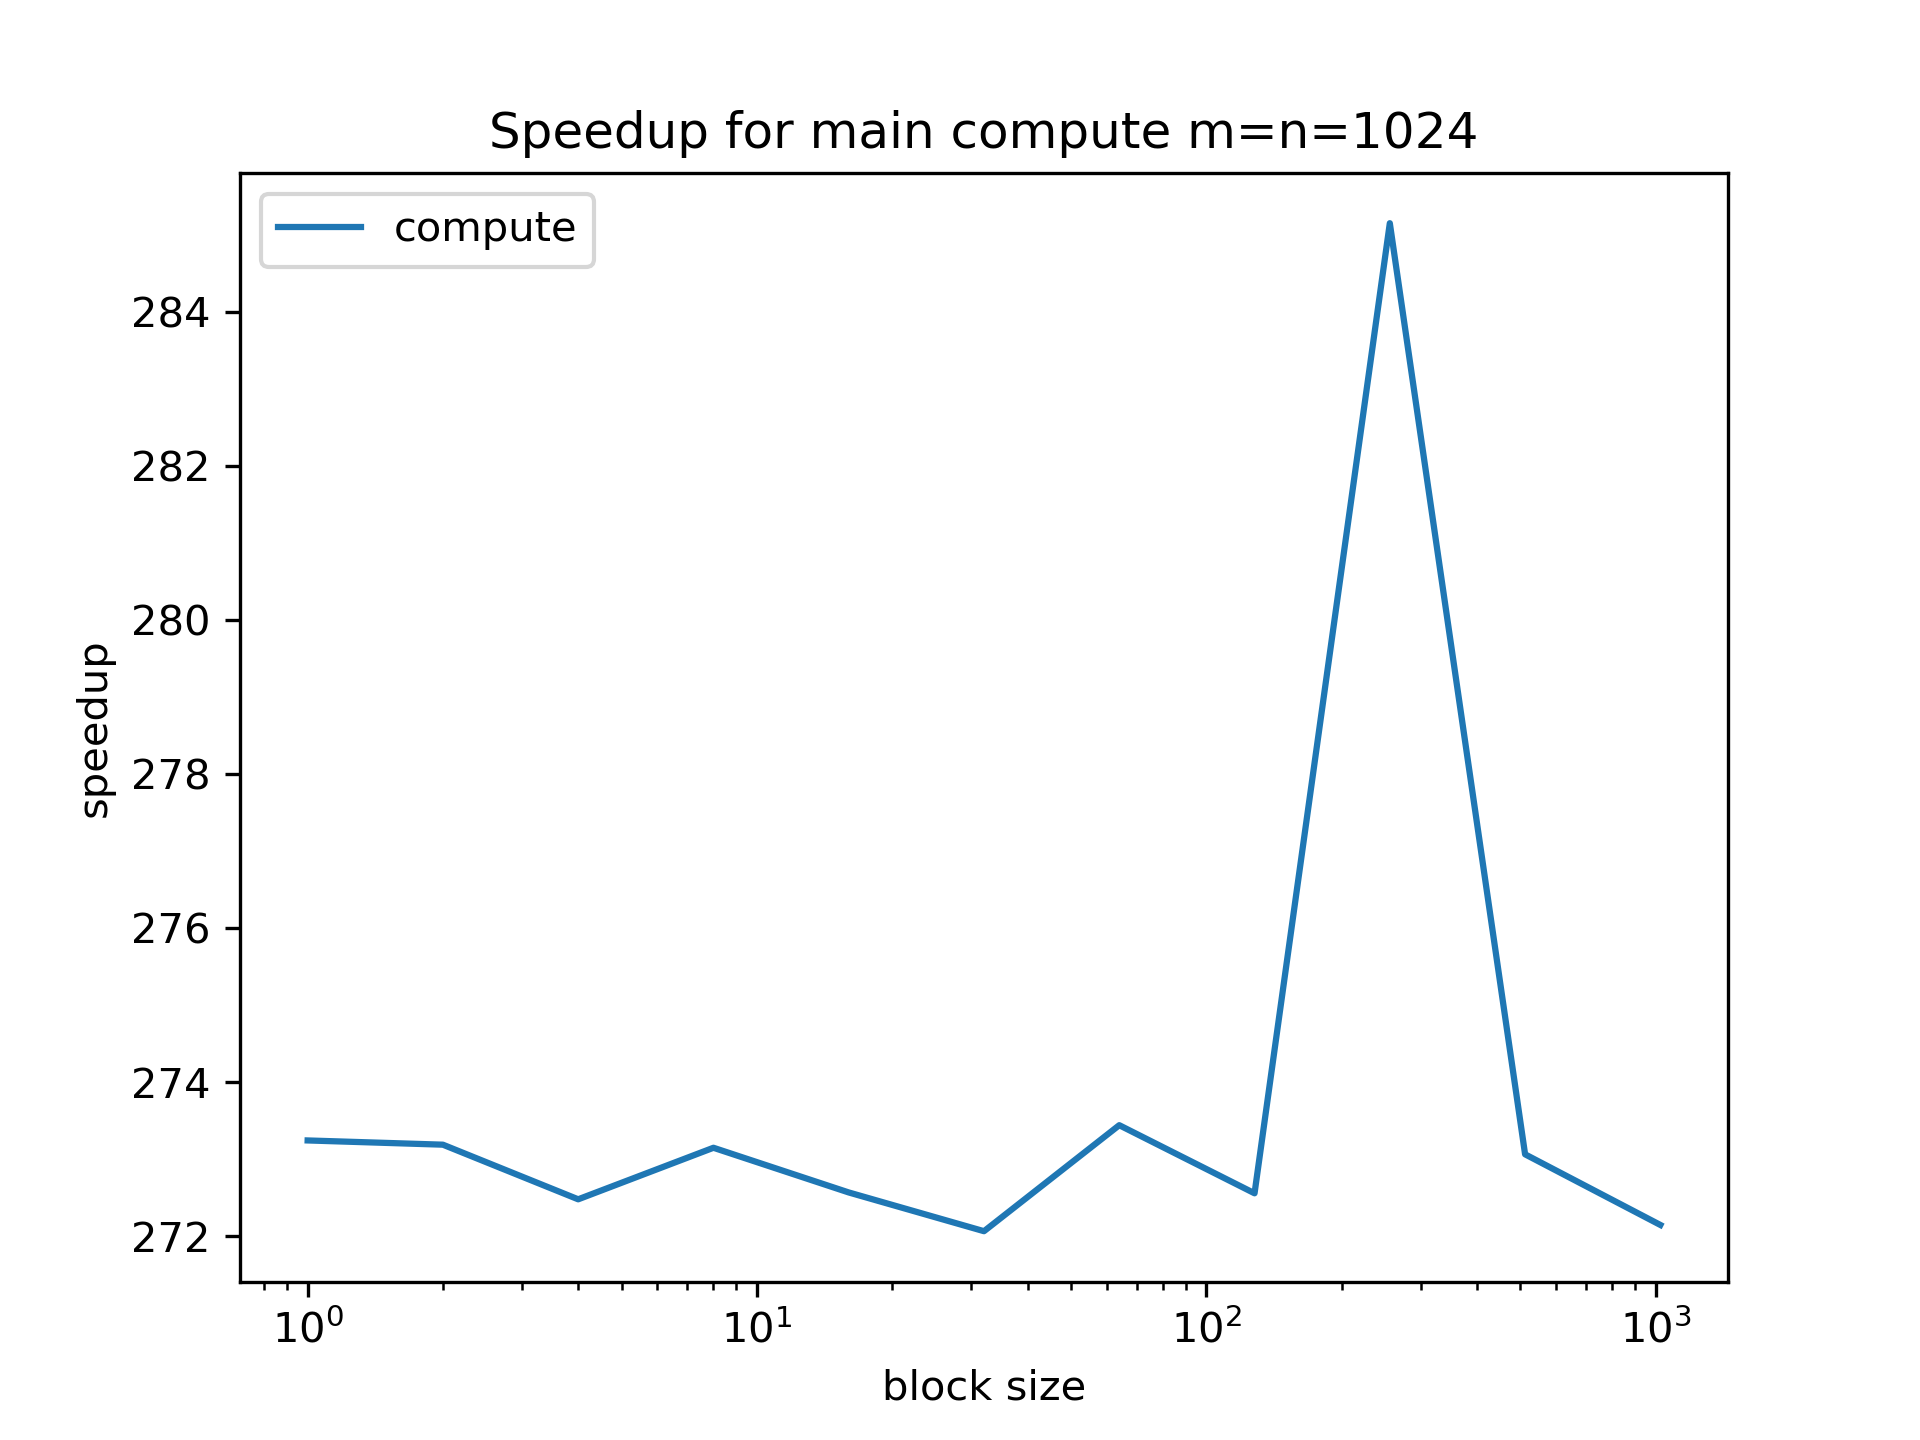
\includegraphics[width=\linewidth]{../float/writeup/compute_plot_m1024.png}
		\end{minipage}%
		\begin{minipage}{0.45\linewidth}
			\centering
			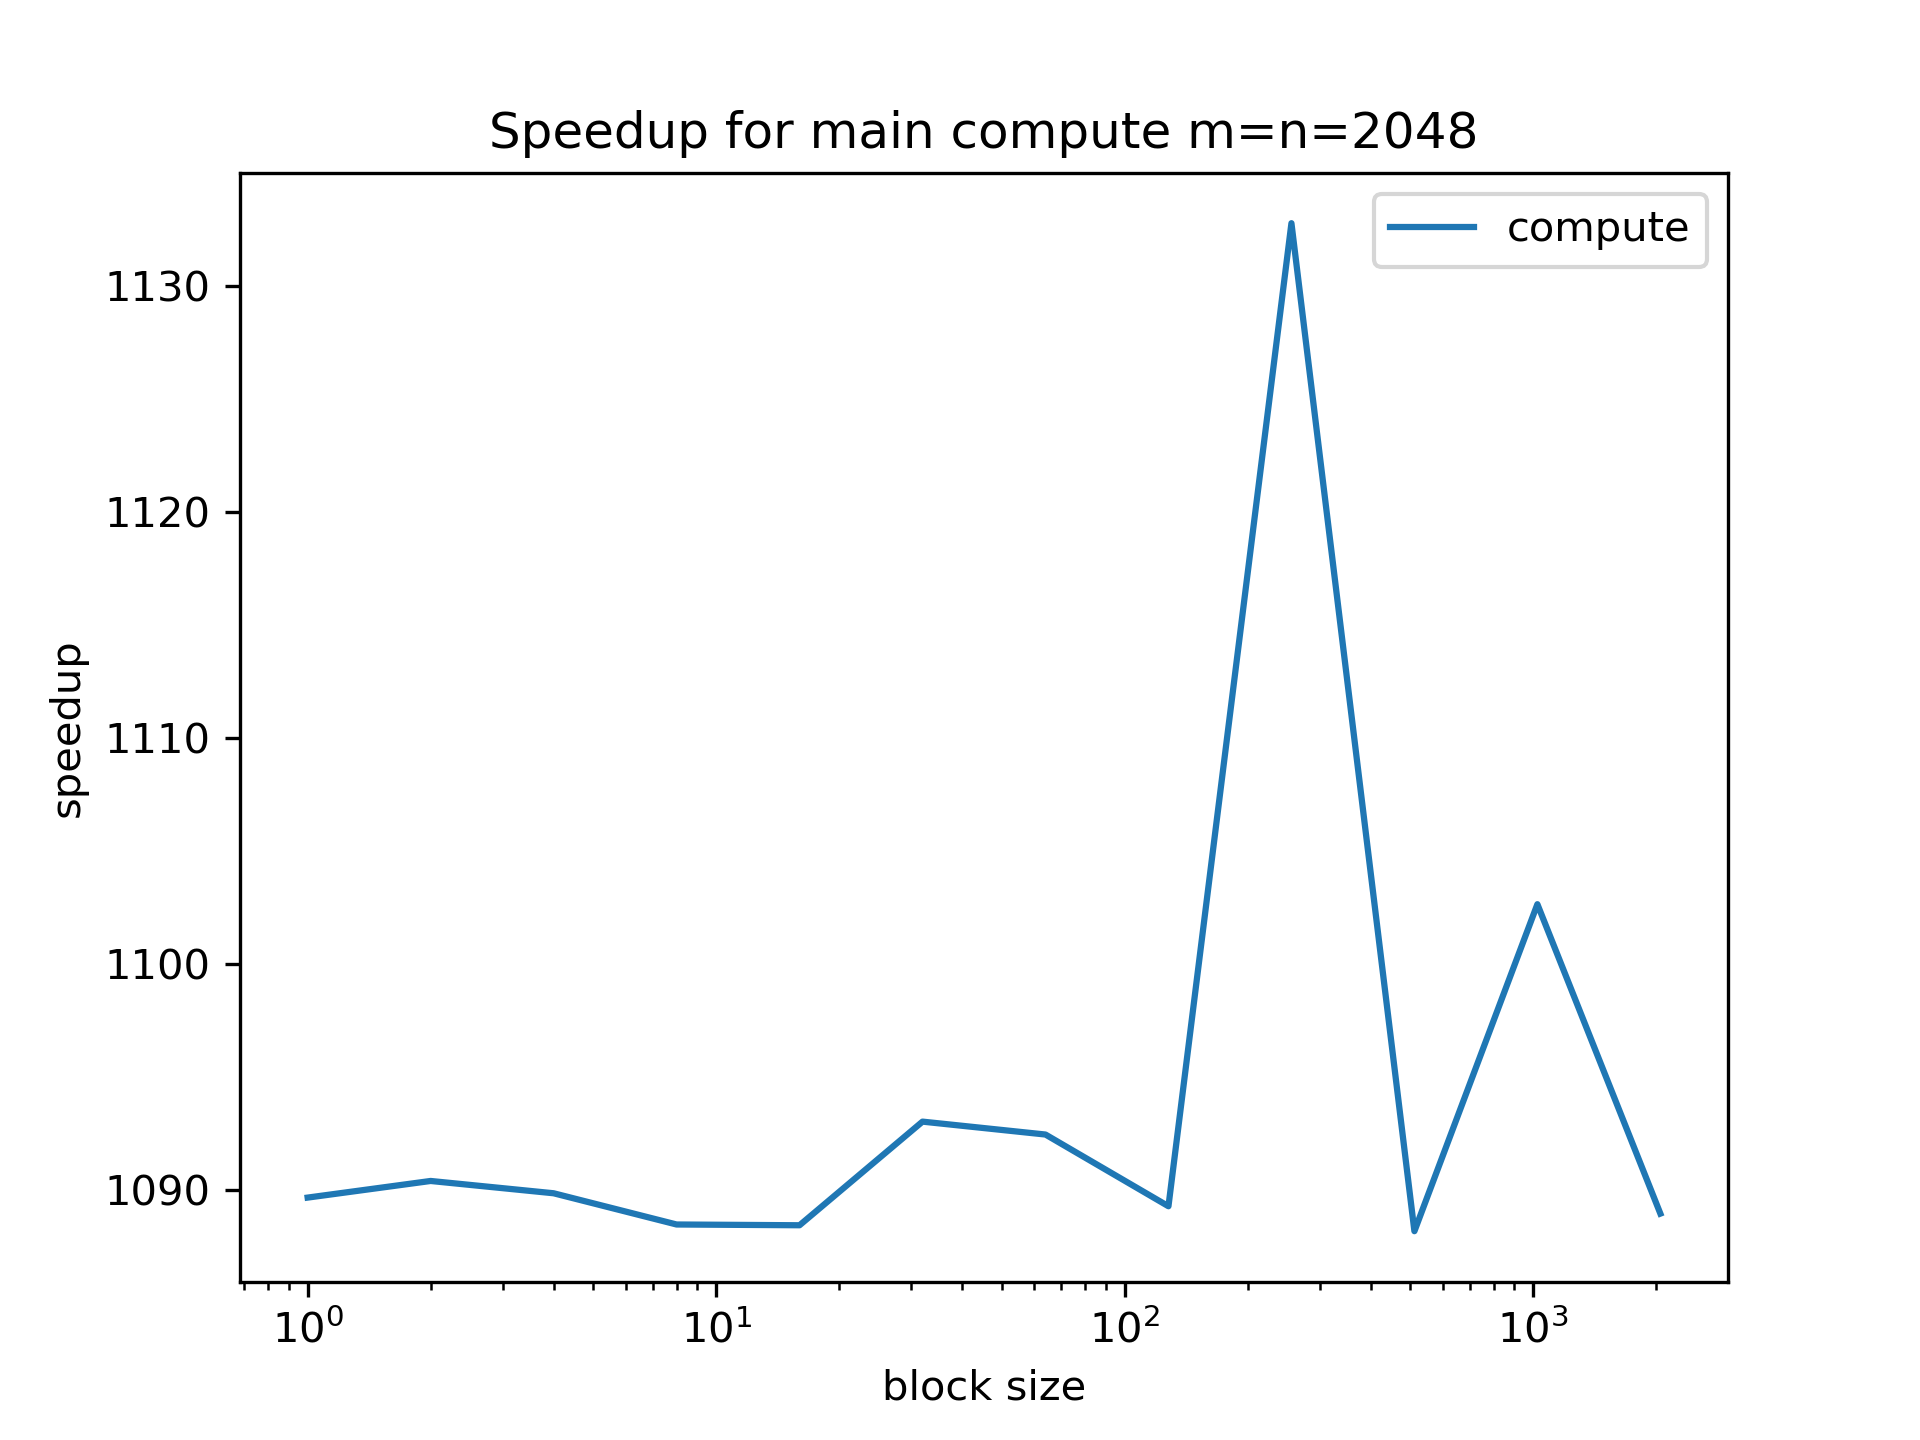
\includegraphics[width=\linewidth]{../float/writeup/compute_plot_m2048.png}
		\end{minipage}
		\vspace{0.5cm} % Adjust the vertical space between rows
		\begin{minipage}{0.45\linewidth}
			\centering
			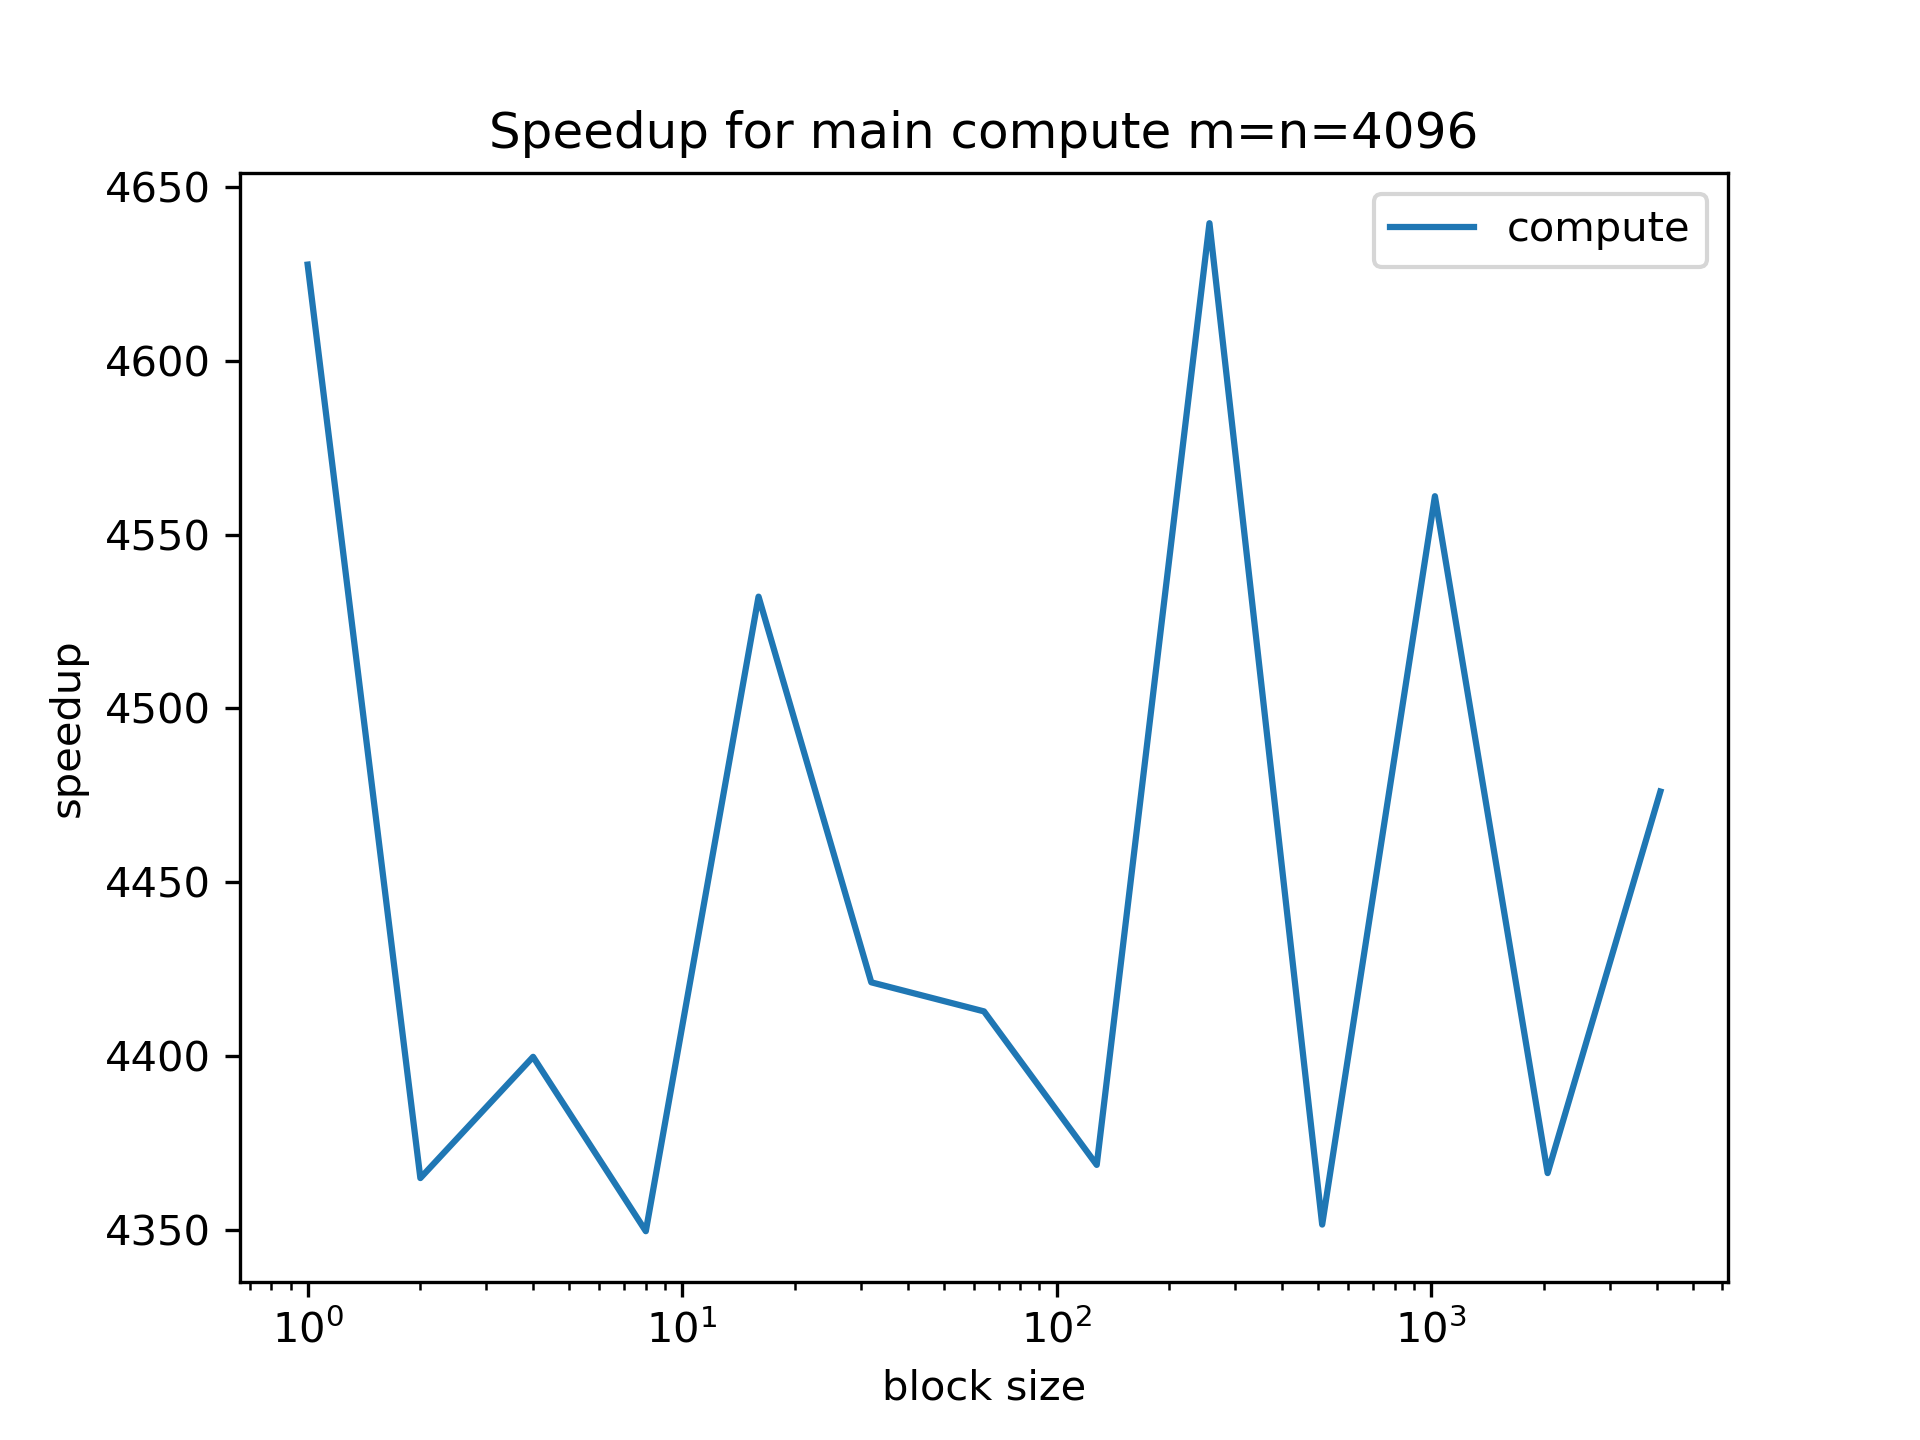
\includegraphics[width=\linewidth]{../float/writeup/compute_plot_m4096.png}
		\end{minipage}%
		\begin{minipage}{0.45\linewidth}
			\centering
			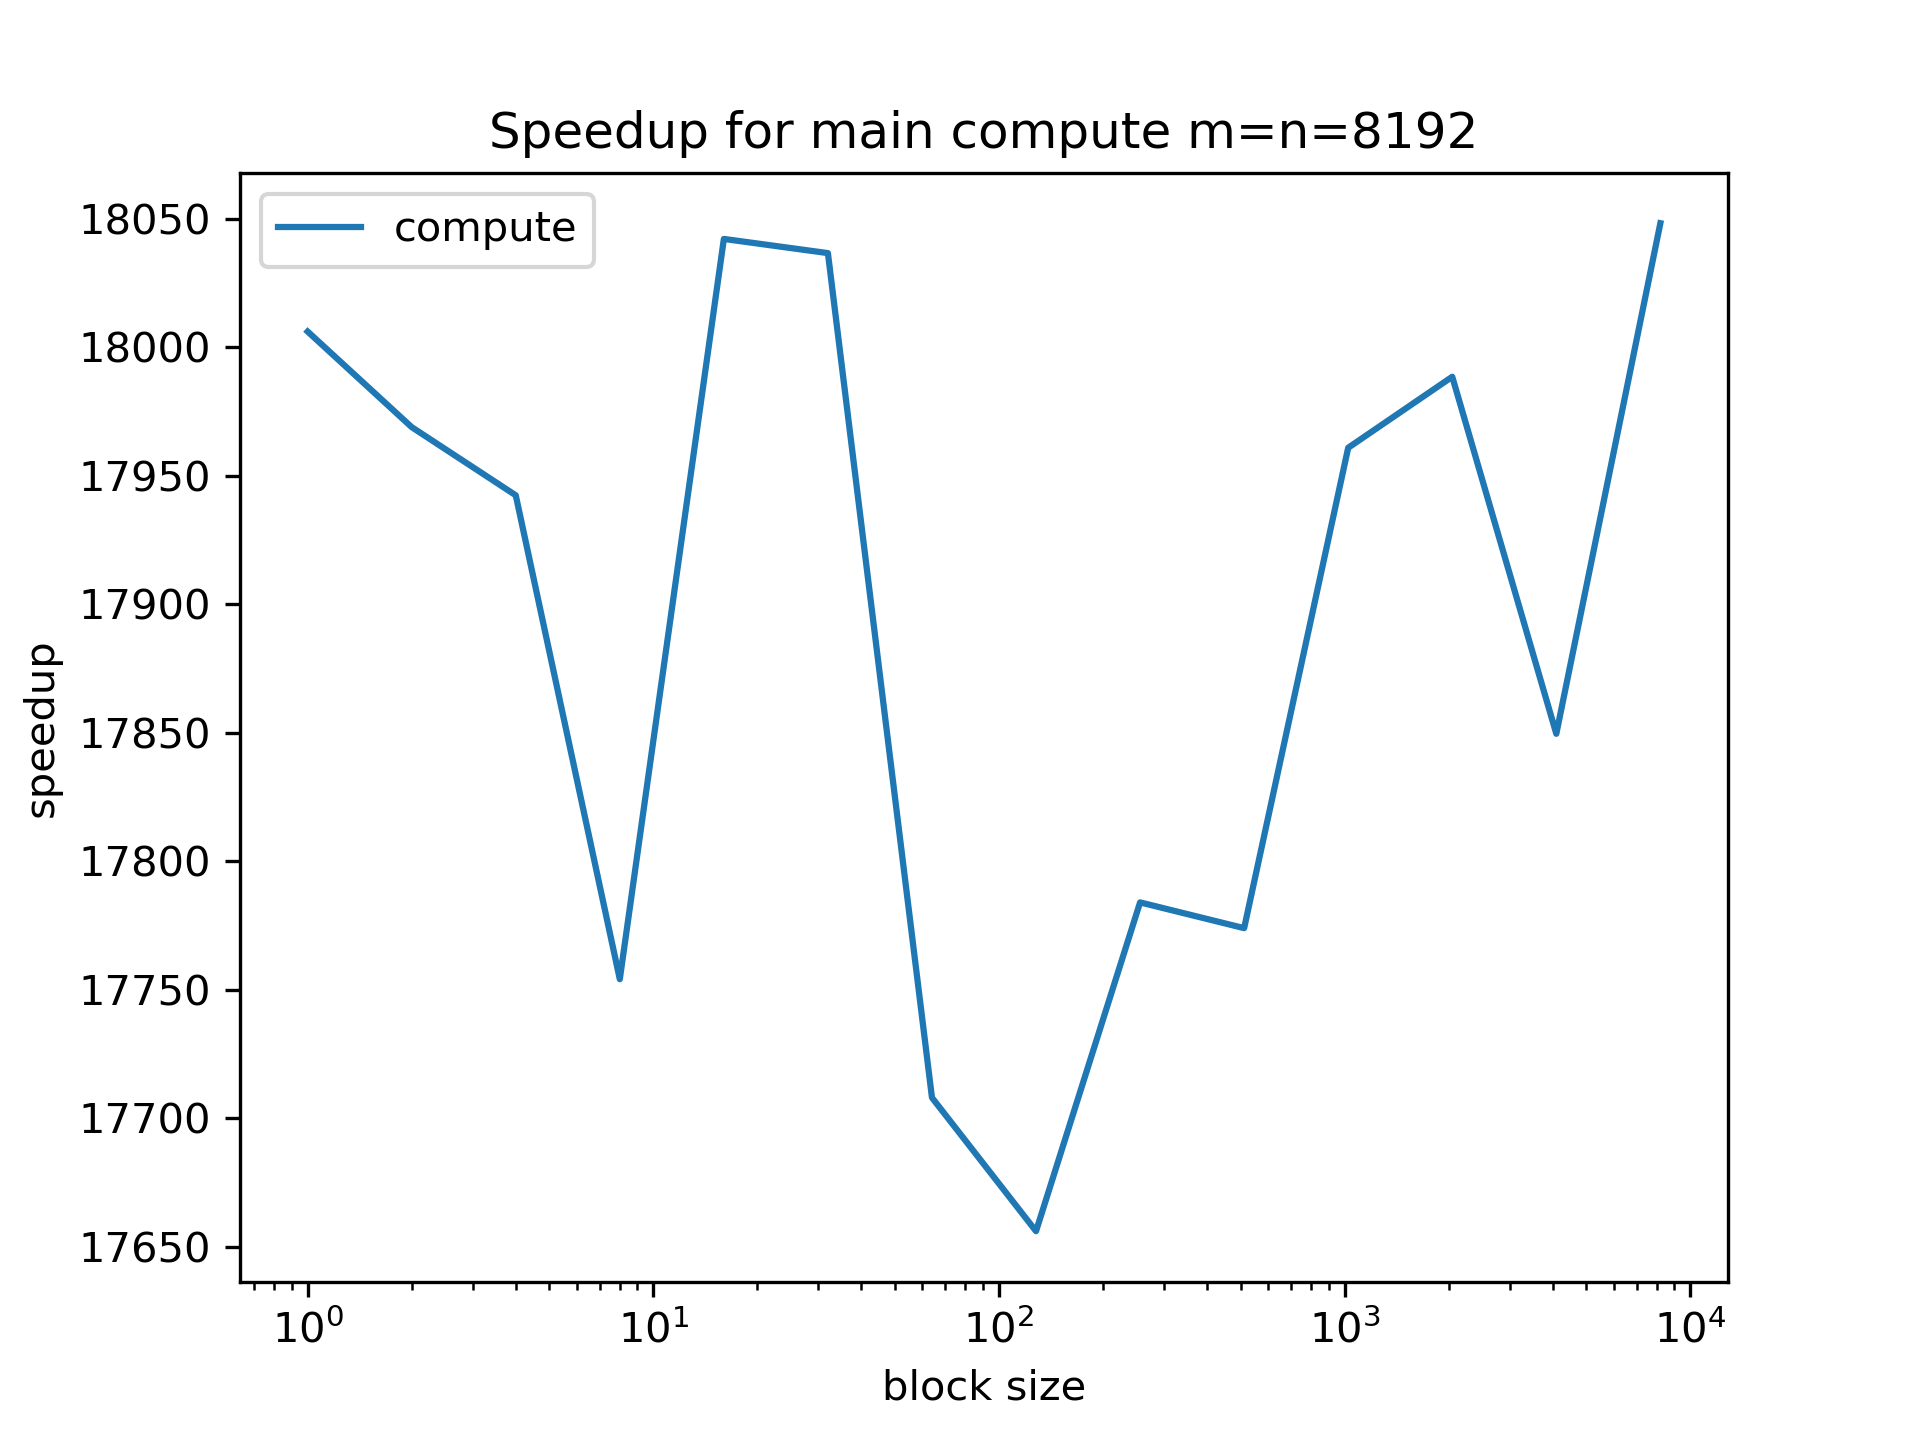
\includegraphics[width=\linewidth]{../float/writeup/compute_plot_m8192.png}
		\end{minipage}
	\end{figure}

		
\section*{Task3}

	In the figure below I plot the speedup against blocksize for the
	caclulation of the average temperature  compared to using my reduction
	code from homework 1. Comparing the performace of both reduction functions,
	there isnt much of a difference. This is probably due to the fact that both 
	functions are using global memory, however, the old one uses a for loop to compute 
	a reduction in a single thread while the new one uses more threads but with an 
	atomic add. I would guess that a sigmificant overhead here is the moving of data
	between threads which doesnt help us in any way. Note a weird spike on the plot
	of matrix $m=n=4096$ in which the simple old code performs waay better. Not sure
	why but I feel that this suggests there could be more improvement in this code. 

	\begin{figure}[h!]
		\centering
		\begin{minipage}{0.45\linewidth}
			\centering
			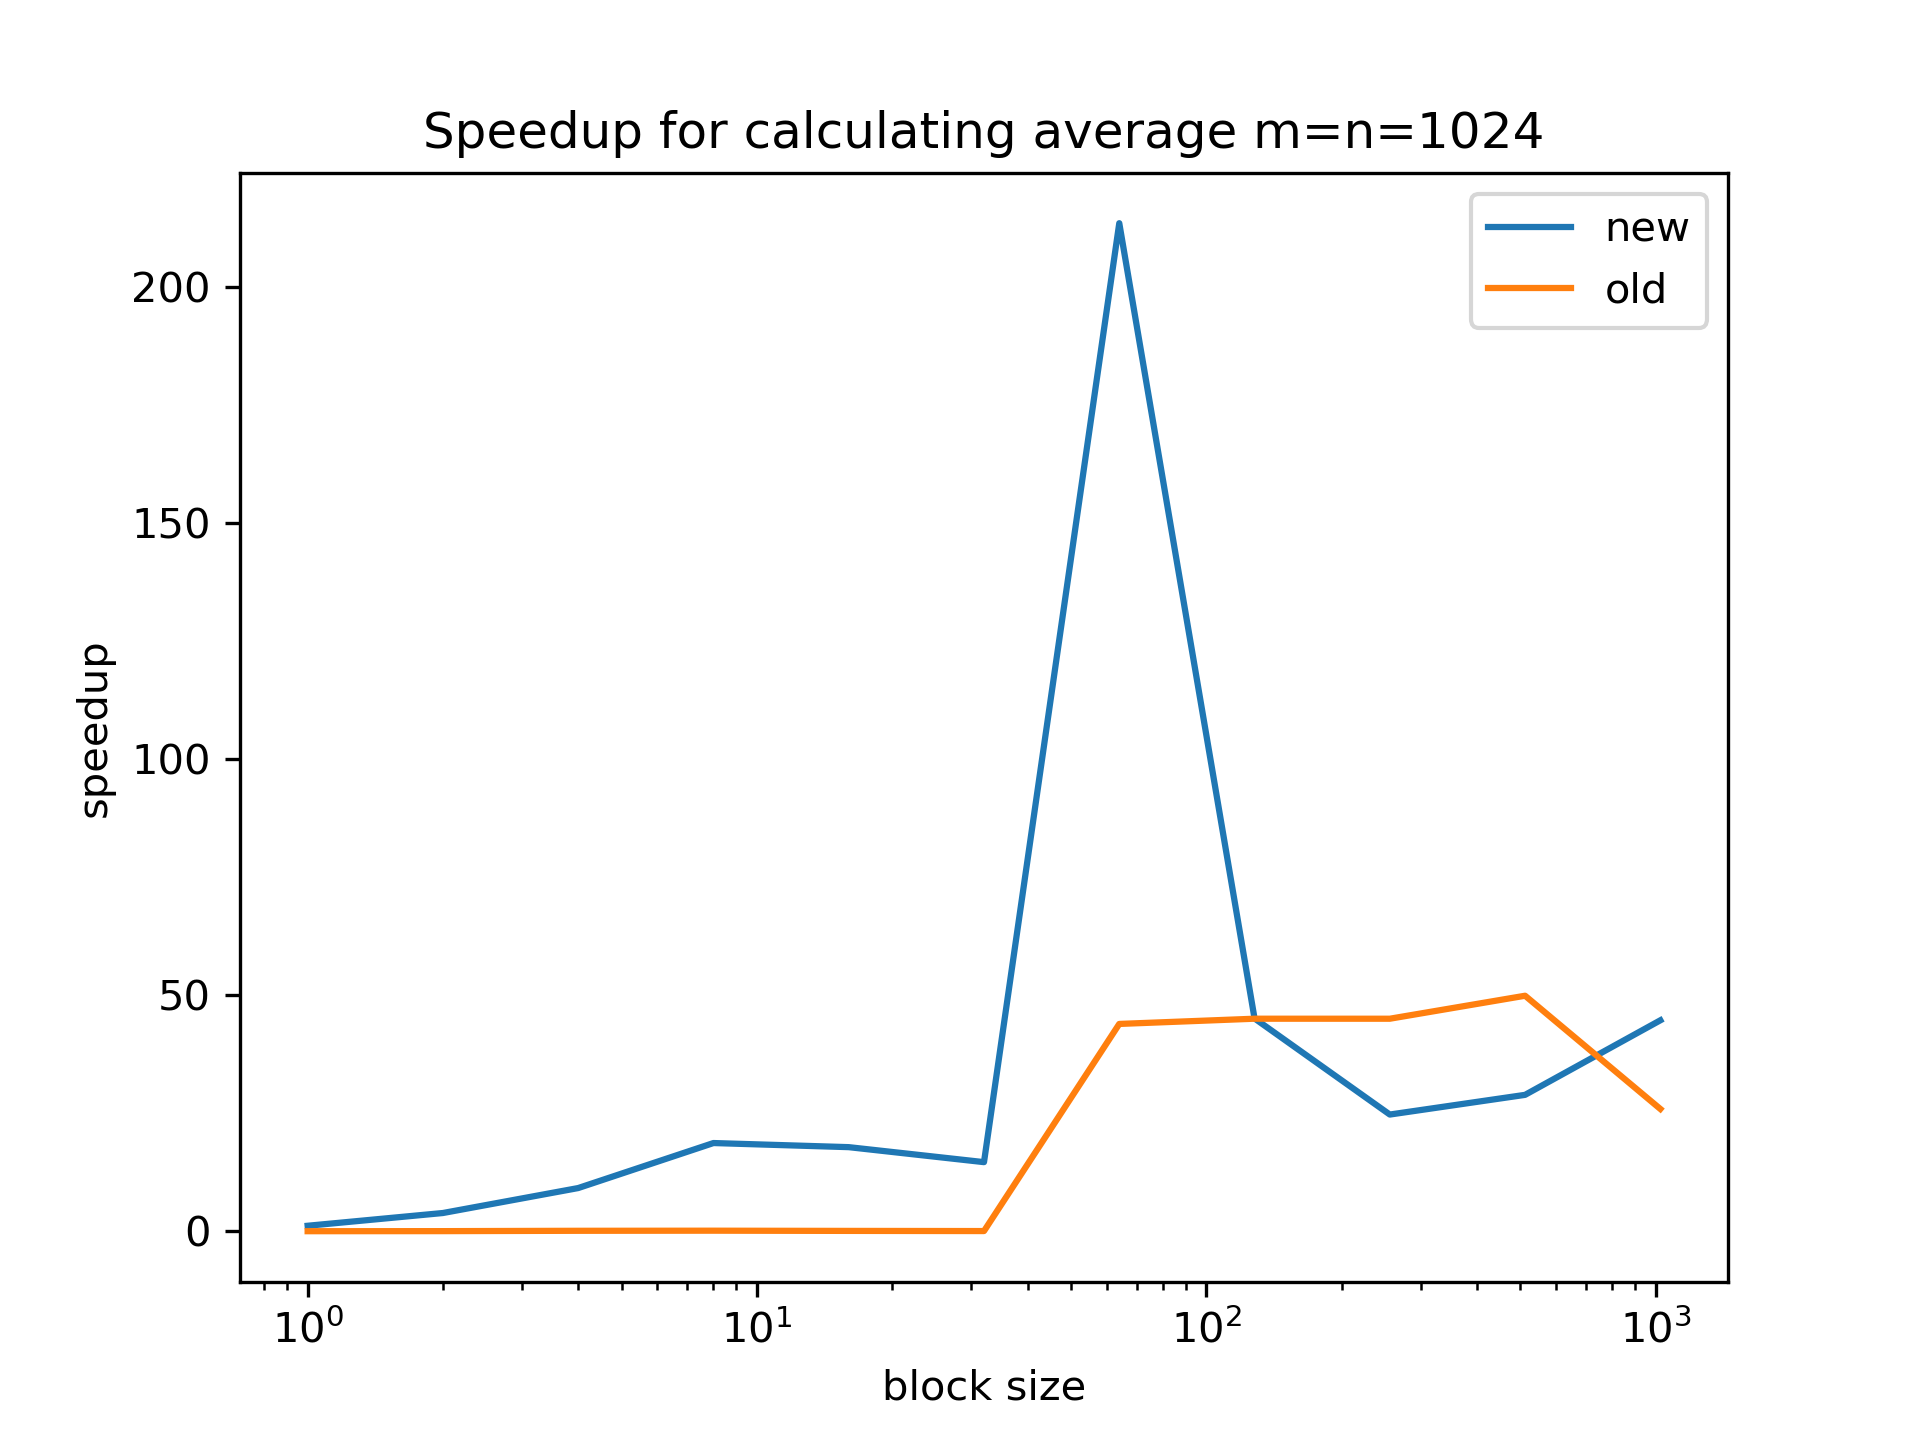
\includegraphics[width=\linewidth]{../float/writeup/reduce_plot_m1024.png}
		\end{minipage}%
		\begin{minipage}{0.45\linewidth}
			\centering
			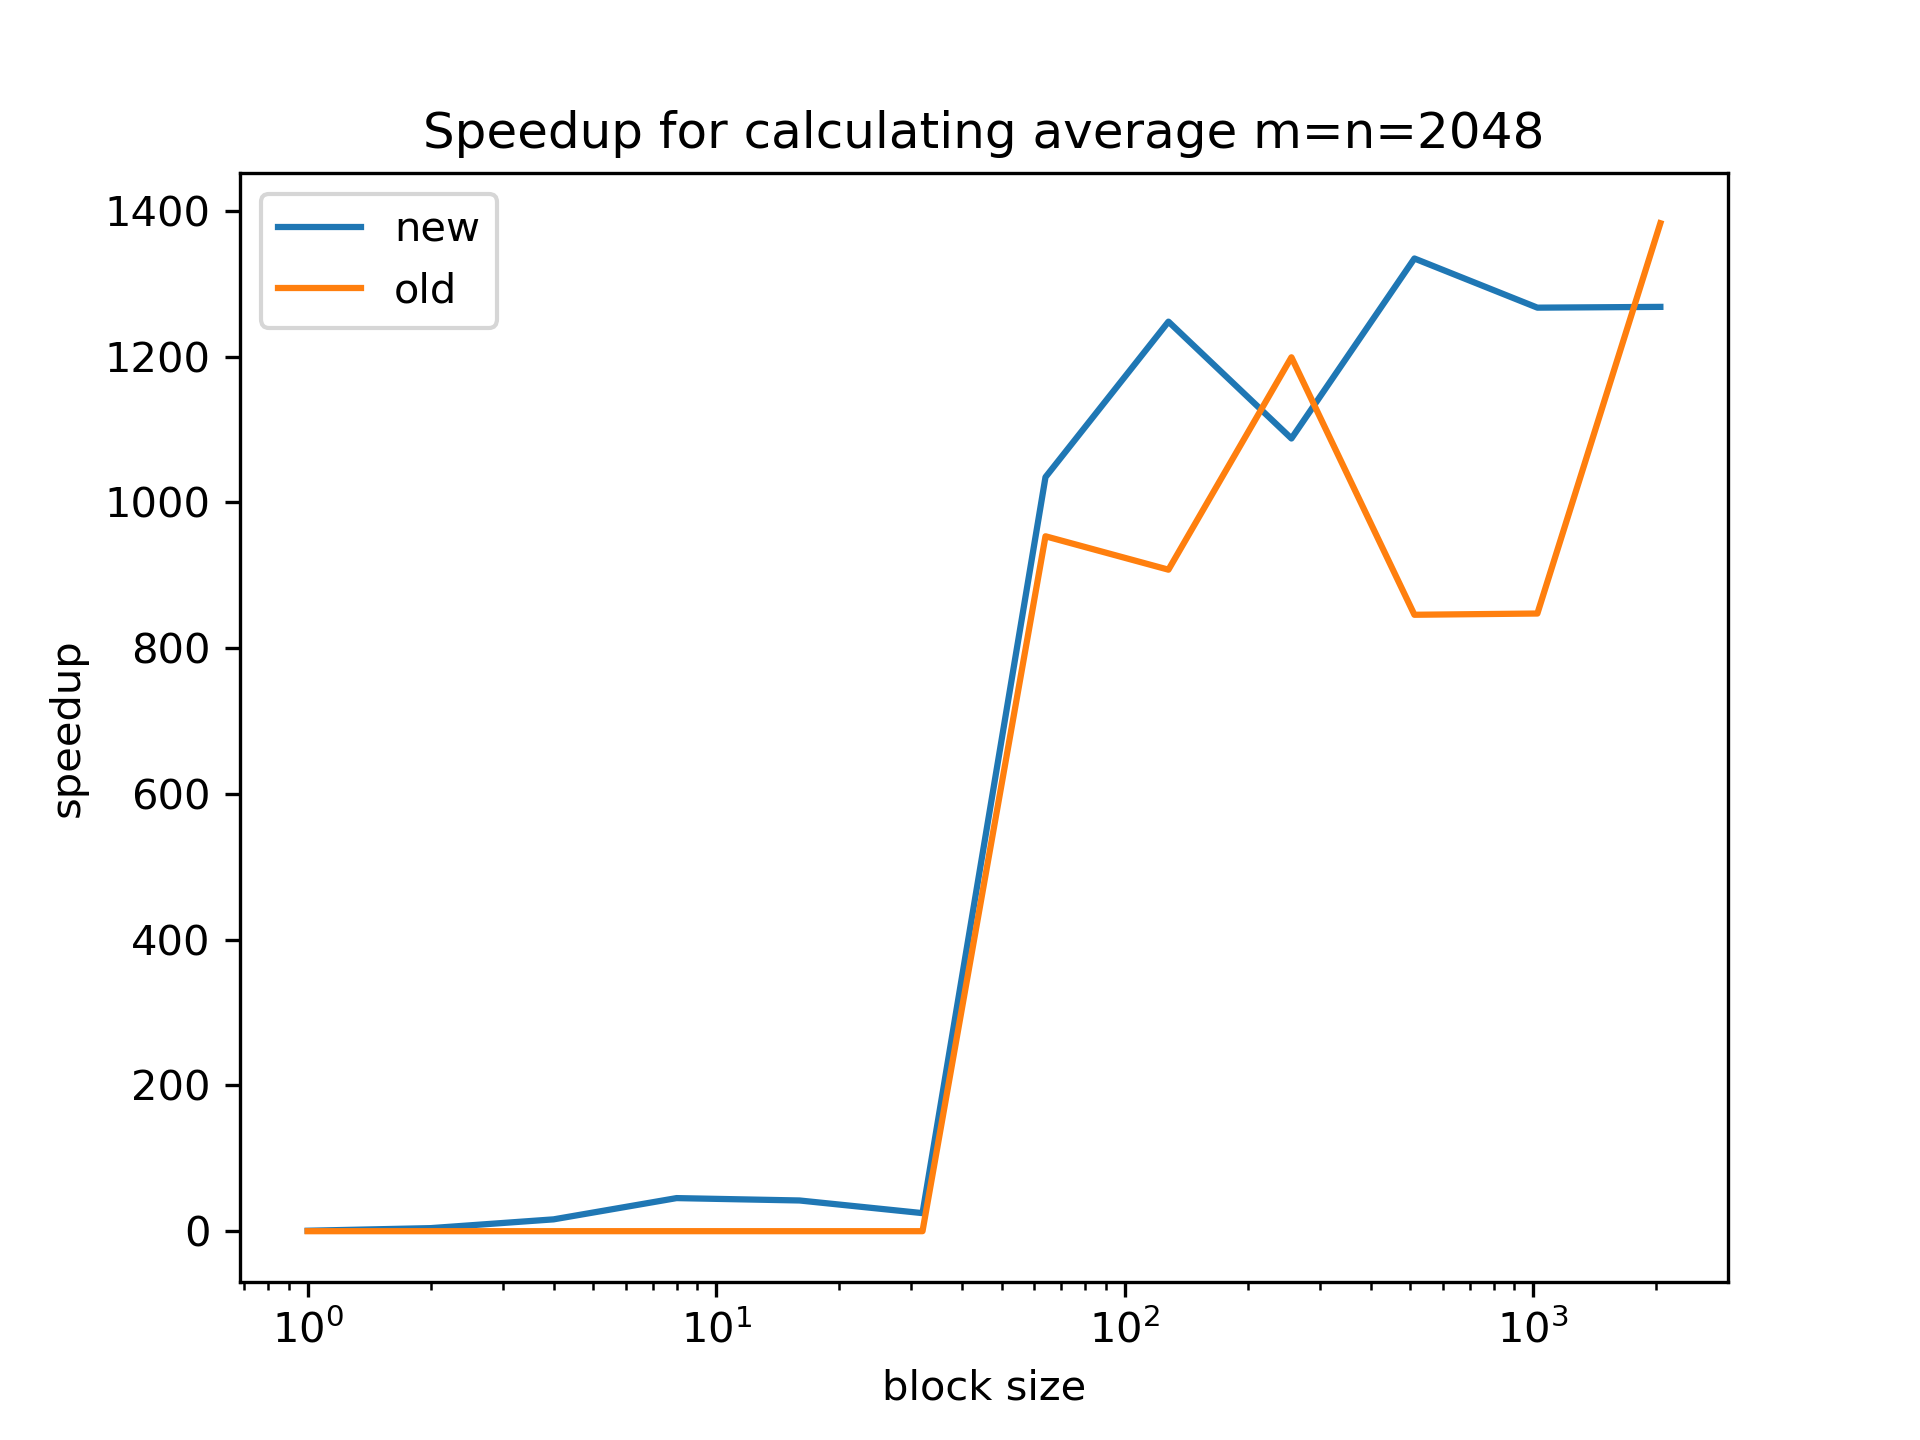
\includegraphics[width=\linewidth]{../float/writeup/reduce_plot_m2048.png}
		\end{minipage}
		\vspace{0.5cm} % Adjust the vertical space between rows
		\begin{minipage}{0.45\linewidth}
			\centering
			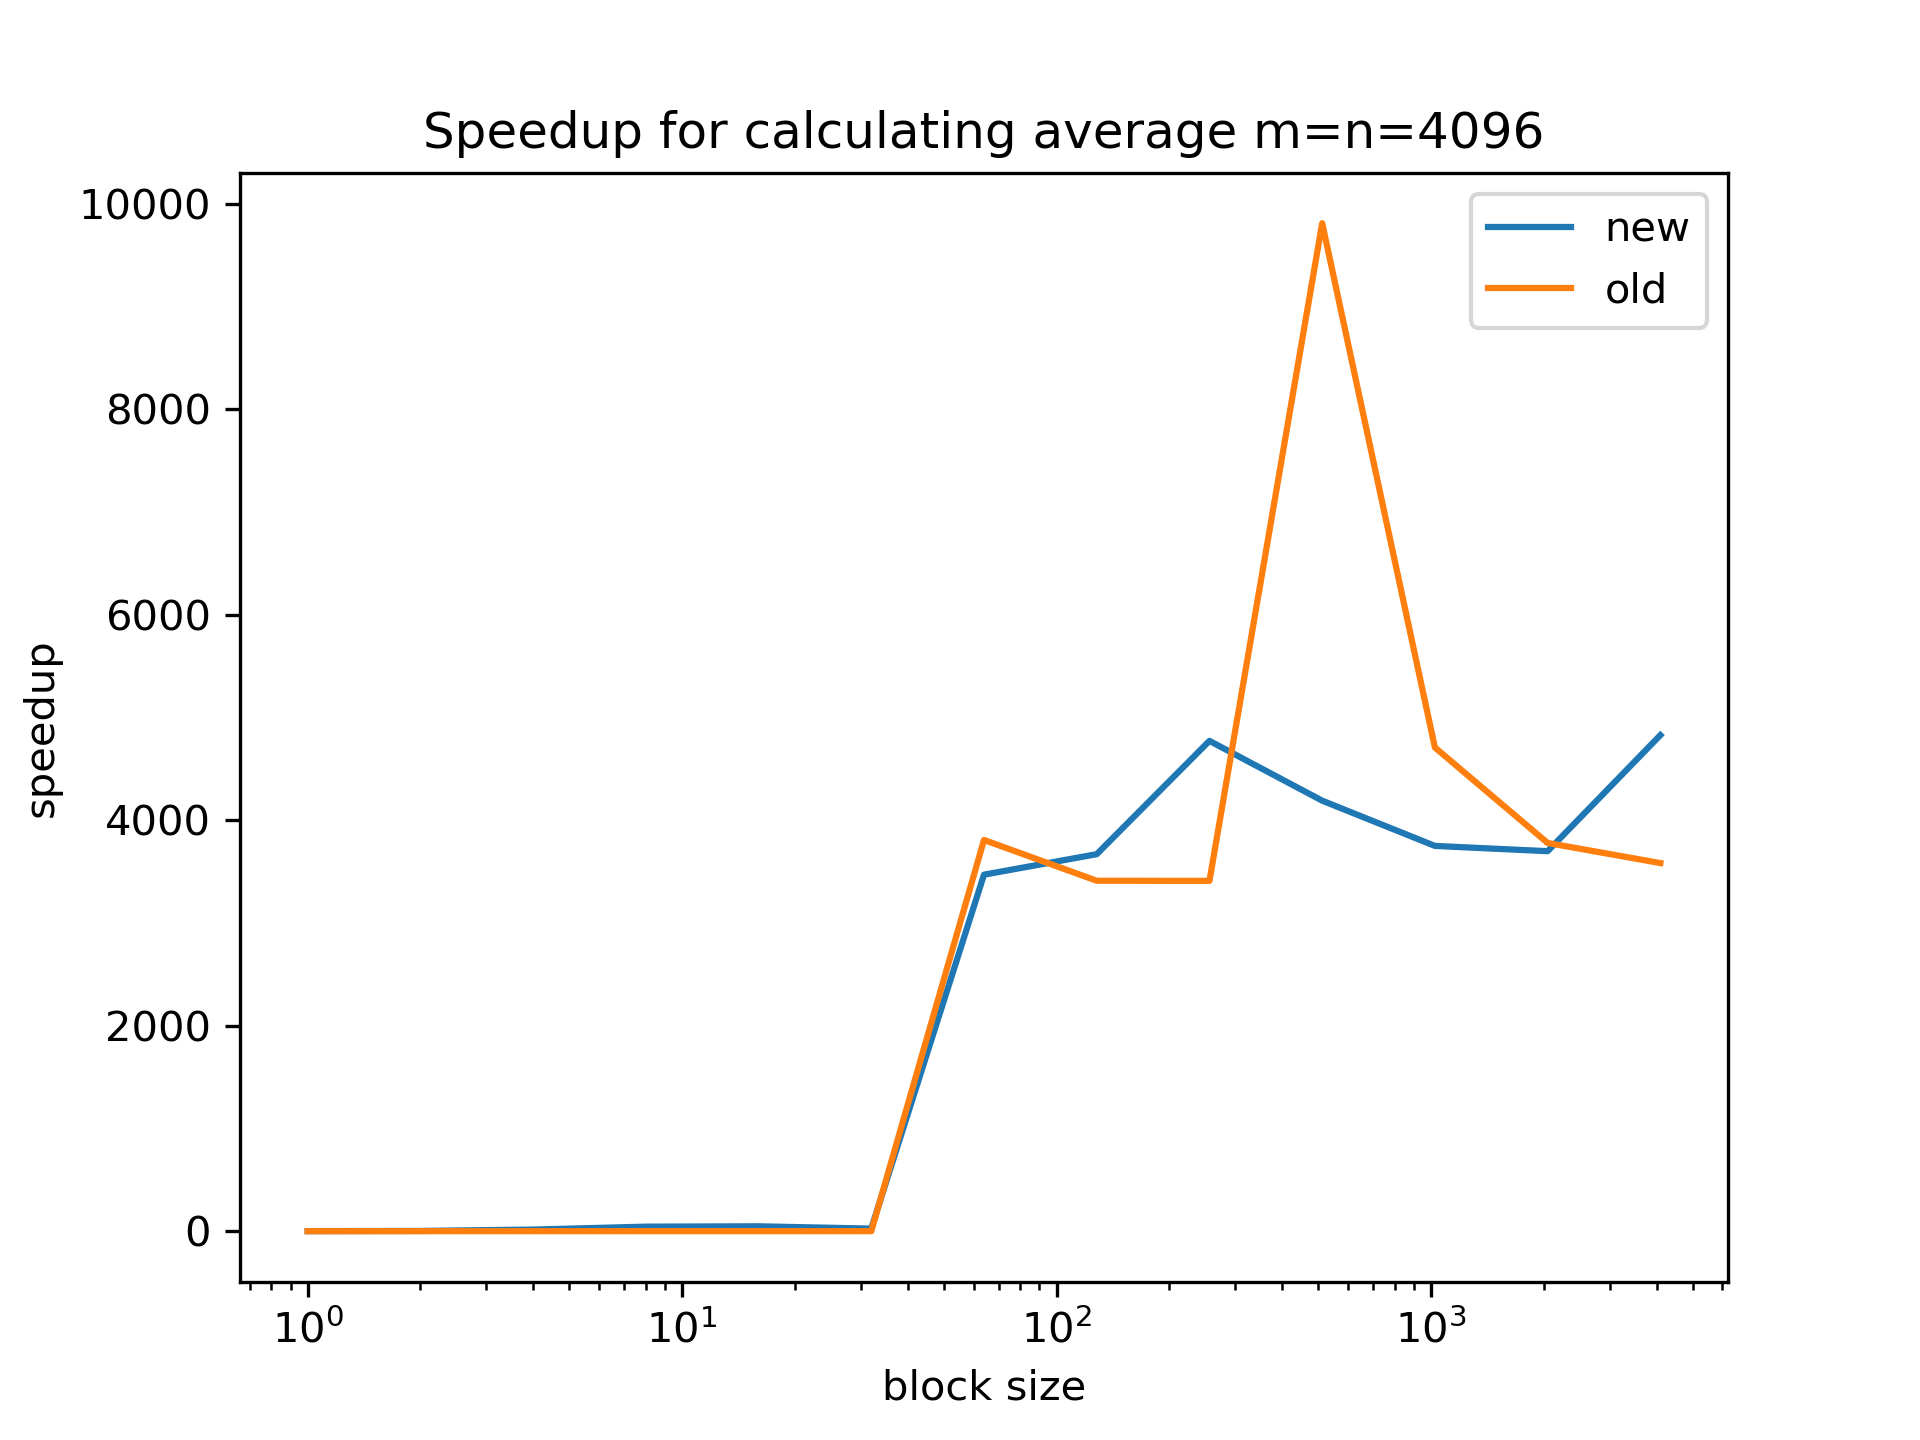
\includegraphics[width=\linewidth]{../float/writeup/reduce_plot_m4096.png}
		\end{minipage}%
		\begin{minipage}{0.45\linewidth}
			\centering
			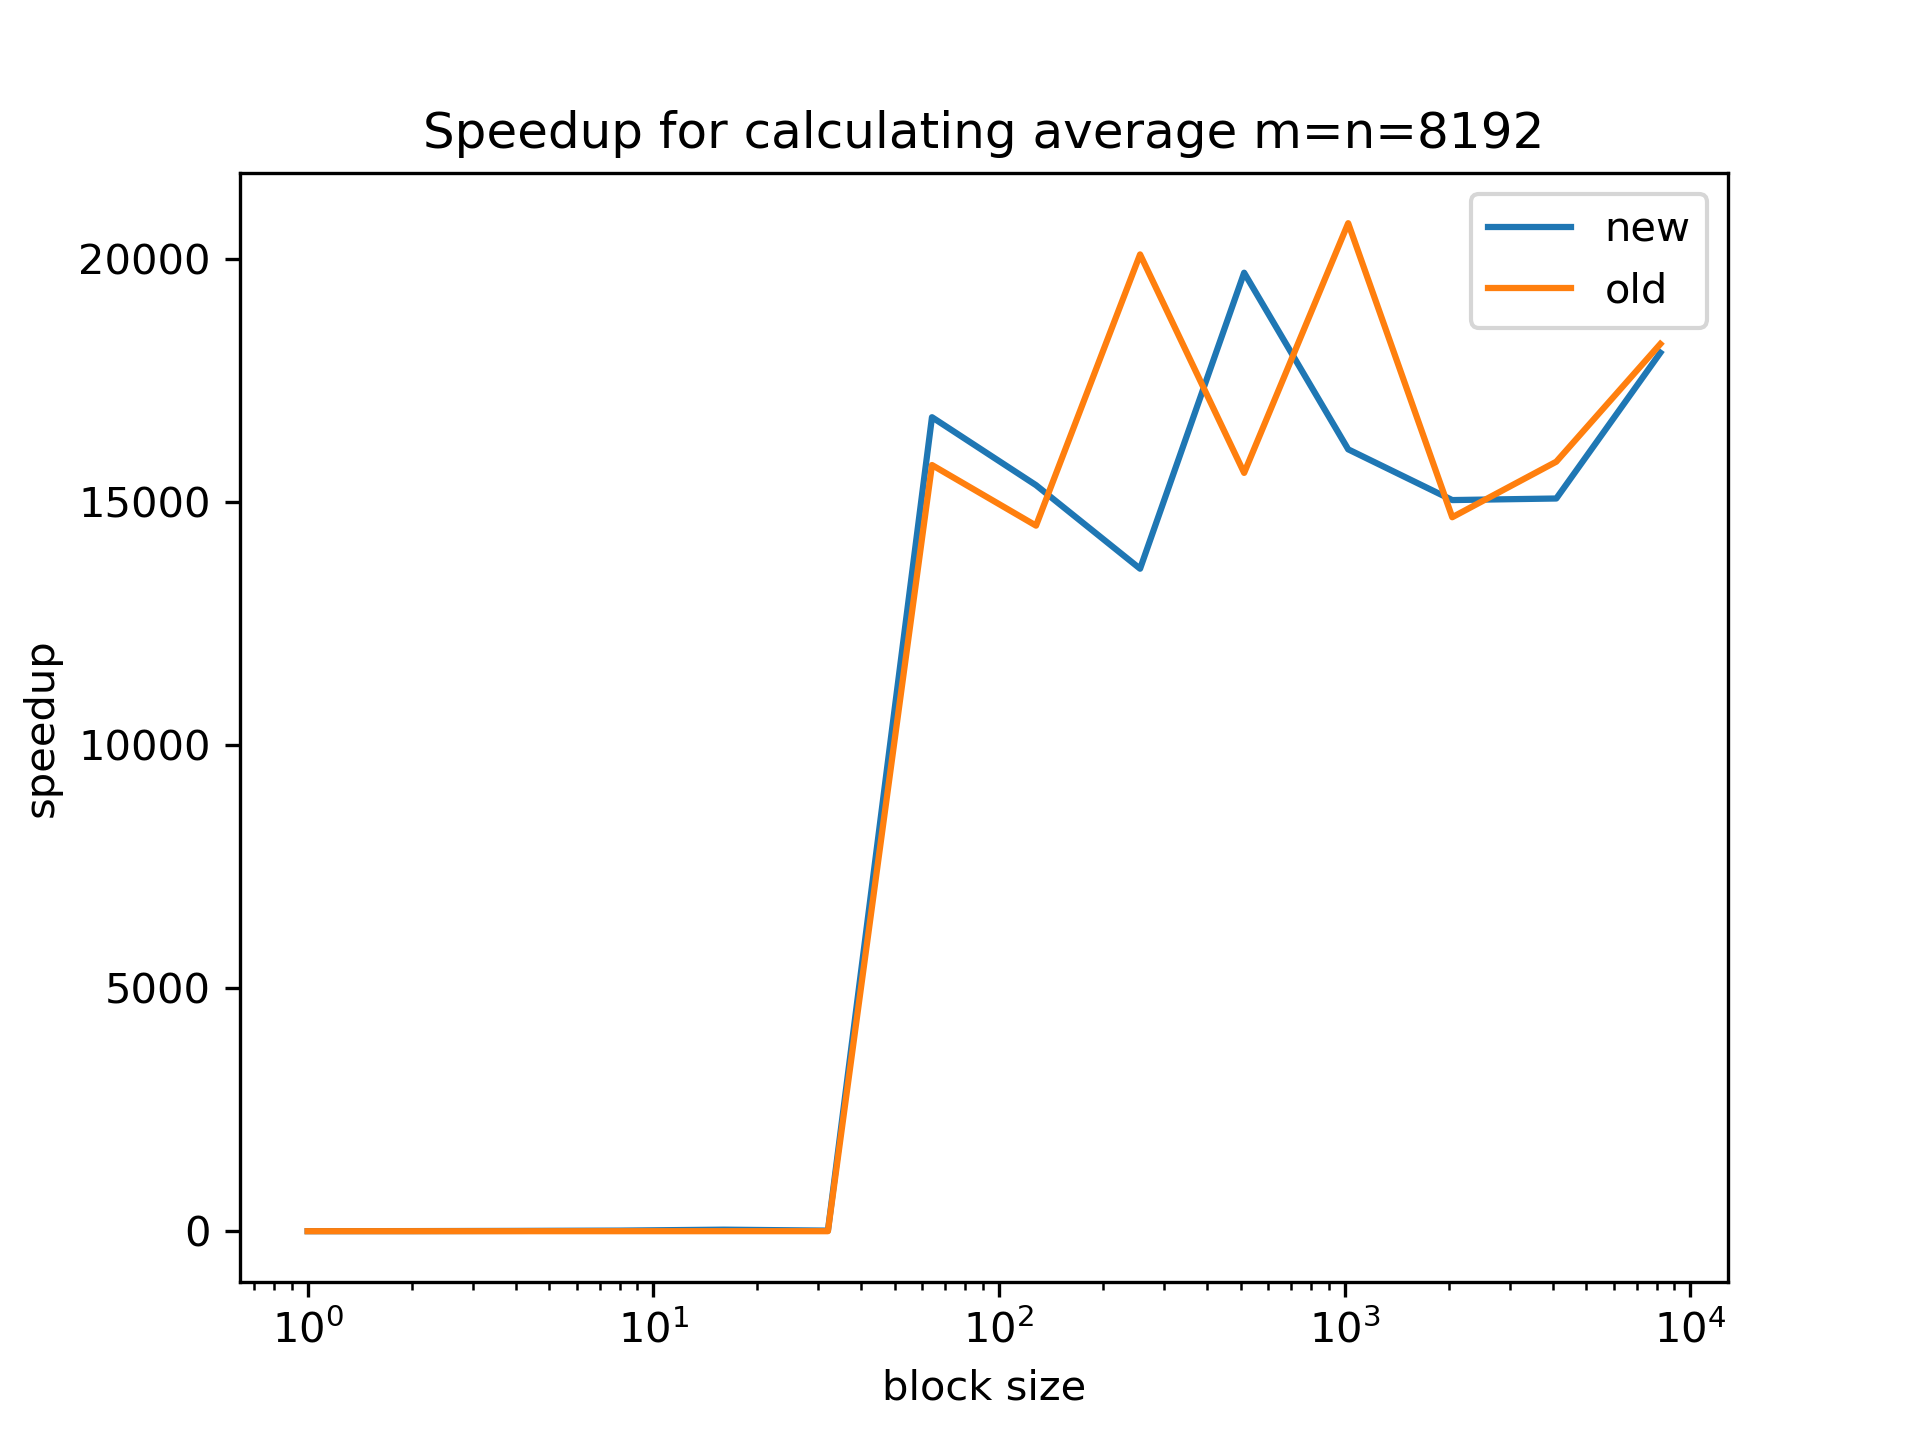
\includegraphics[width=\linewidth]{../float/writeup/reduce_plot_m8192.png}
		\end{minipage}
	\end{figure}


\section*{Task4}
	
	For this task involving converting the cuda code into double precision I wasnt able
	to completely convert the main iteration loop as surface memory which I was using 
	to store my matrices cant hold double precision numbers easily. Instead I chose to 
	only change the main computation in double precision while storing the results in 
	floating point precision by downcasting the results into floats. Replacing the floats
	with doubles in every other bit of code otherwise worked without much thought.

	Below are plots comparing the float and double code. The results are as expected,
	that is the double code takes longer than the float code in the case of the main
	compute however the speedup for the reduction for calcualting averages is mostly the
	same and the lines intersect eachother which I would say is due to minor differences
	in the condition of the whole machine with other people runing code at the same time. 
	
	\begin{figure}[h!]
		\centering
		\begin{minipage}{0.45\linewidth}
			\centering
			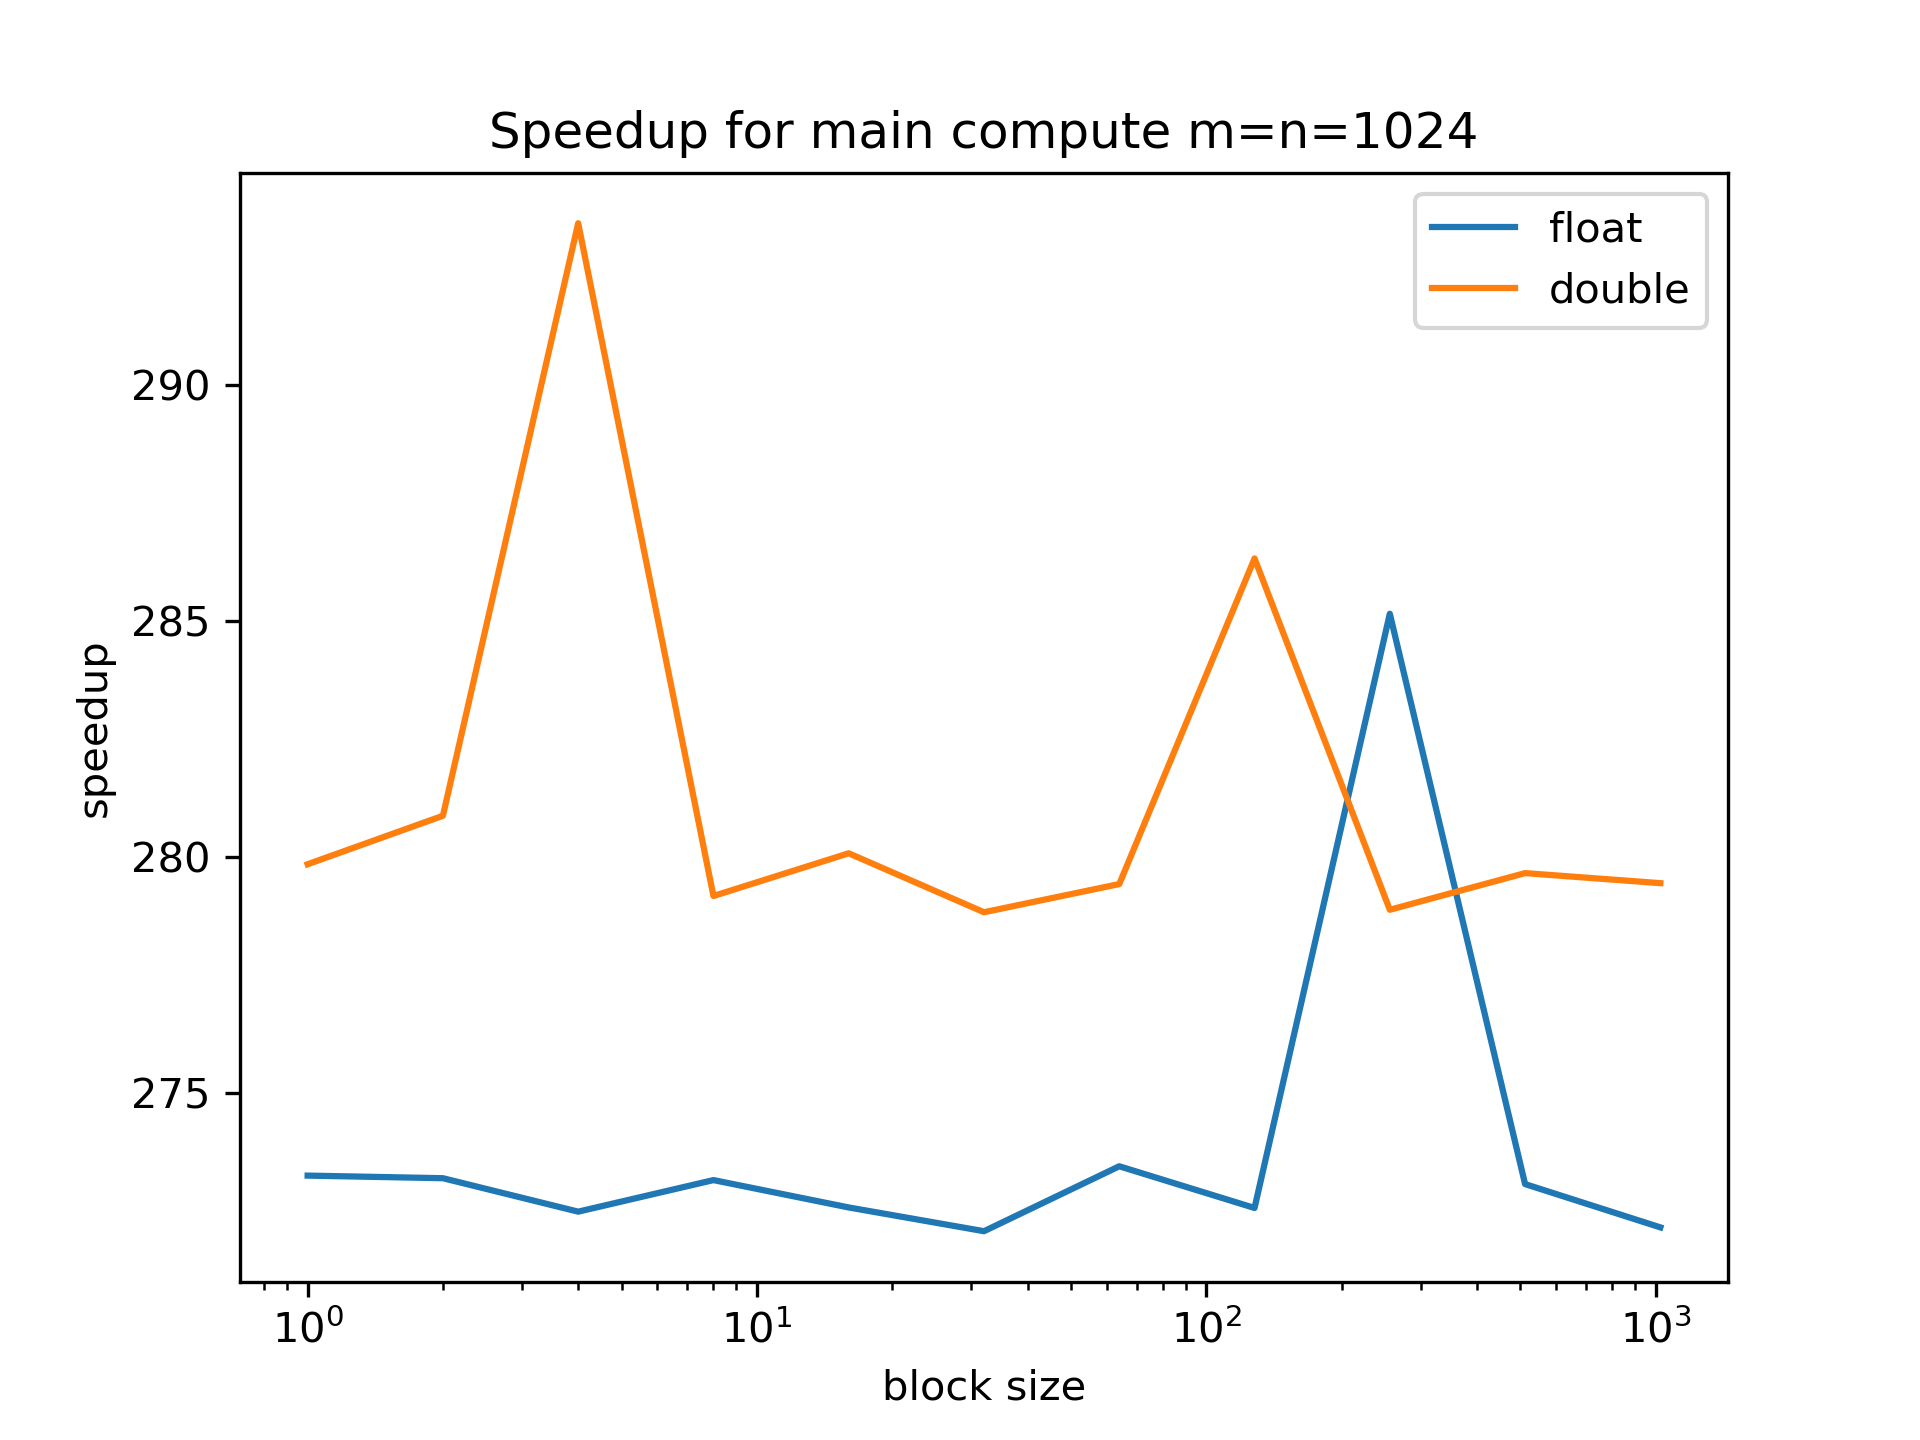
\includegraphics[width=\linewidth]{../comparison_plots/compute_plot_m1024.png}
		\end{minipage}%
		\begin{minipage}{0.45\linewidth}
			\centering
			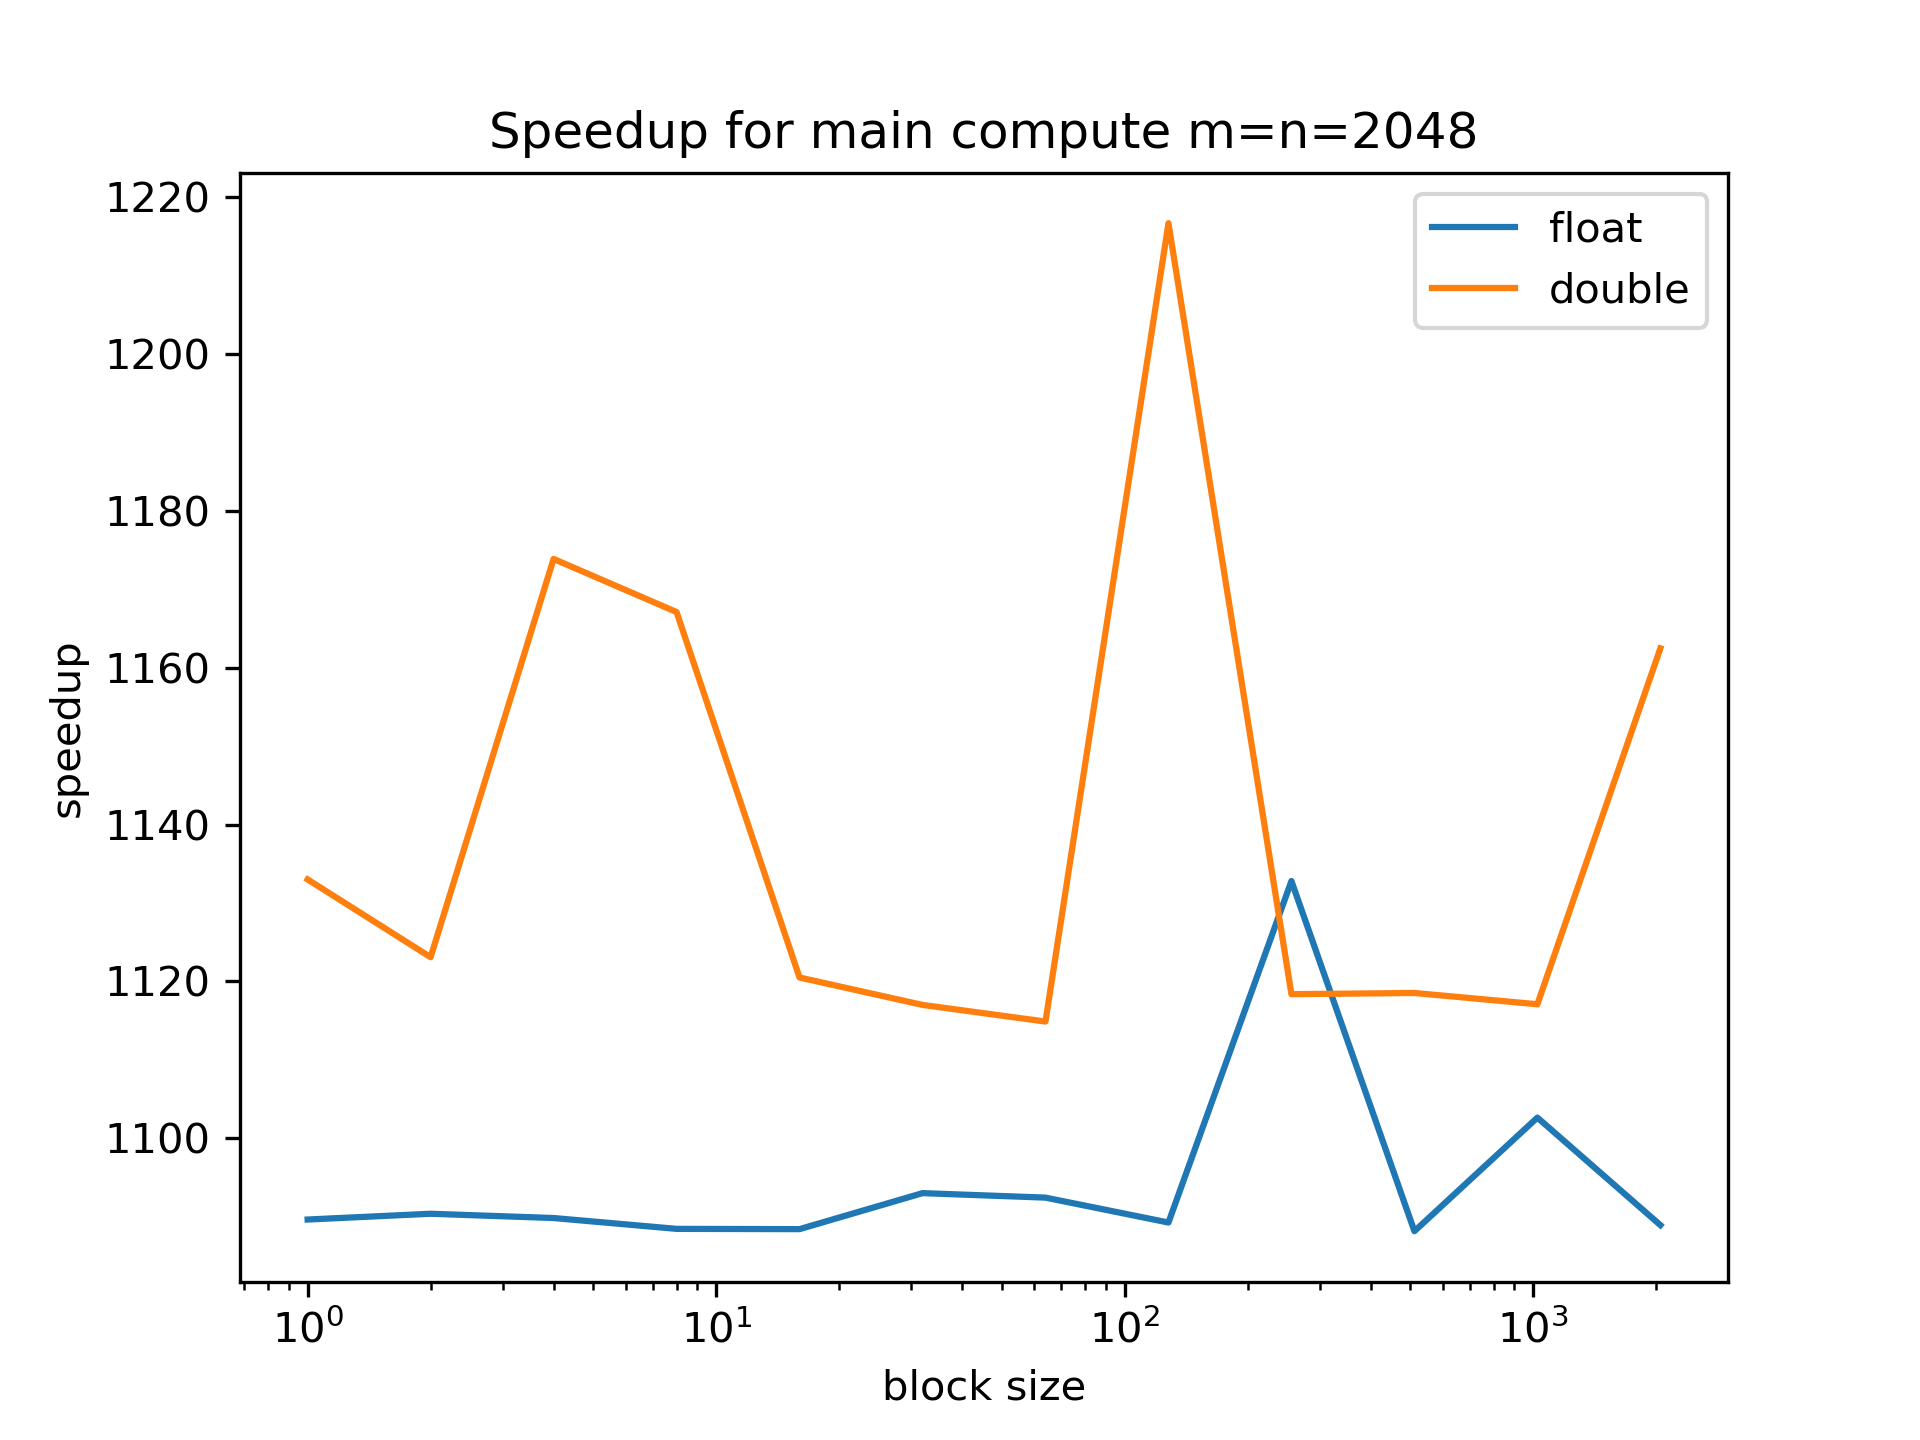
\includegraphics[width=\linewidth]{../comparison_plots/compute_plot_m2048.png}
		\end{minipage}
		\vspace{0.5cm} % Adjust the vertical space between rows
		\begin{minipage}{0.45\linewidth}
			\centering
			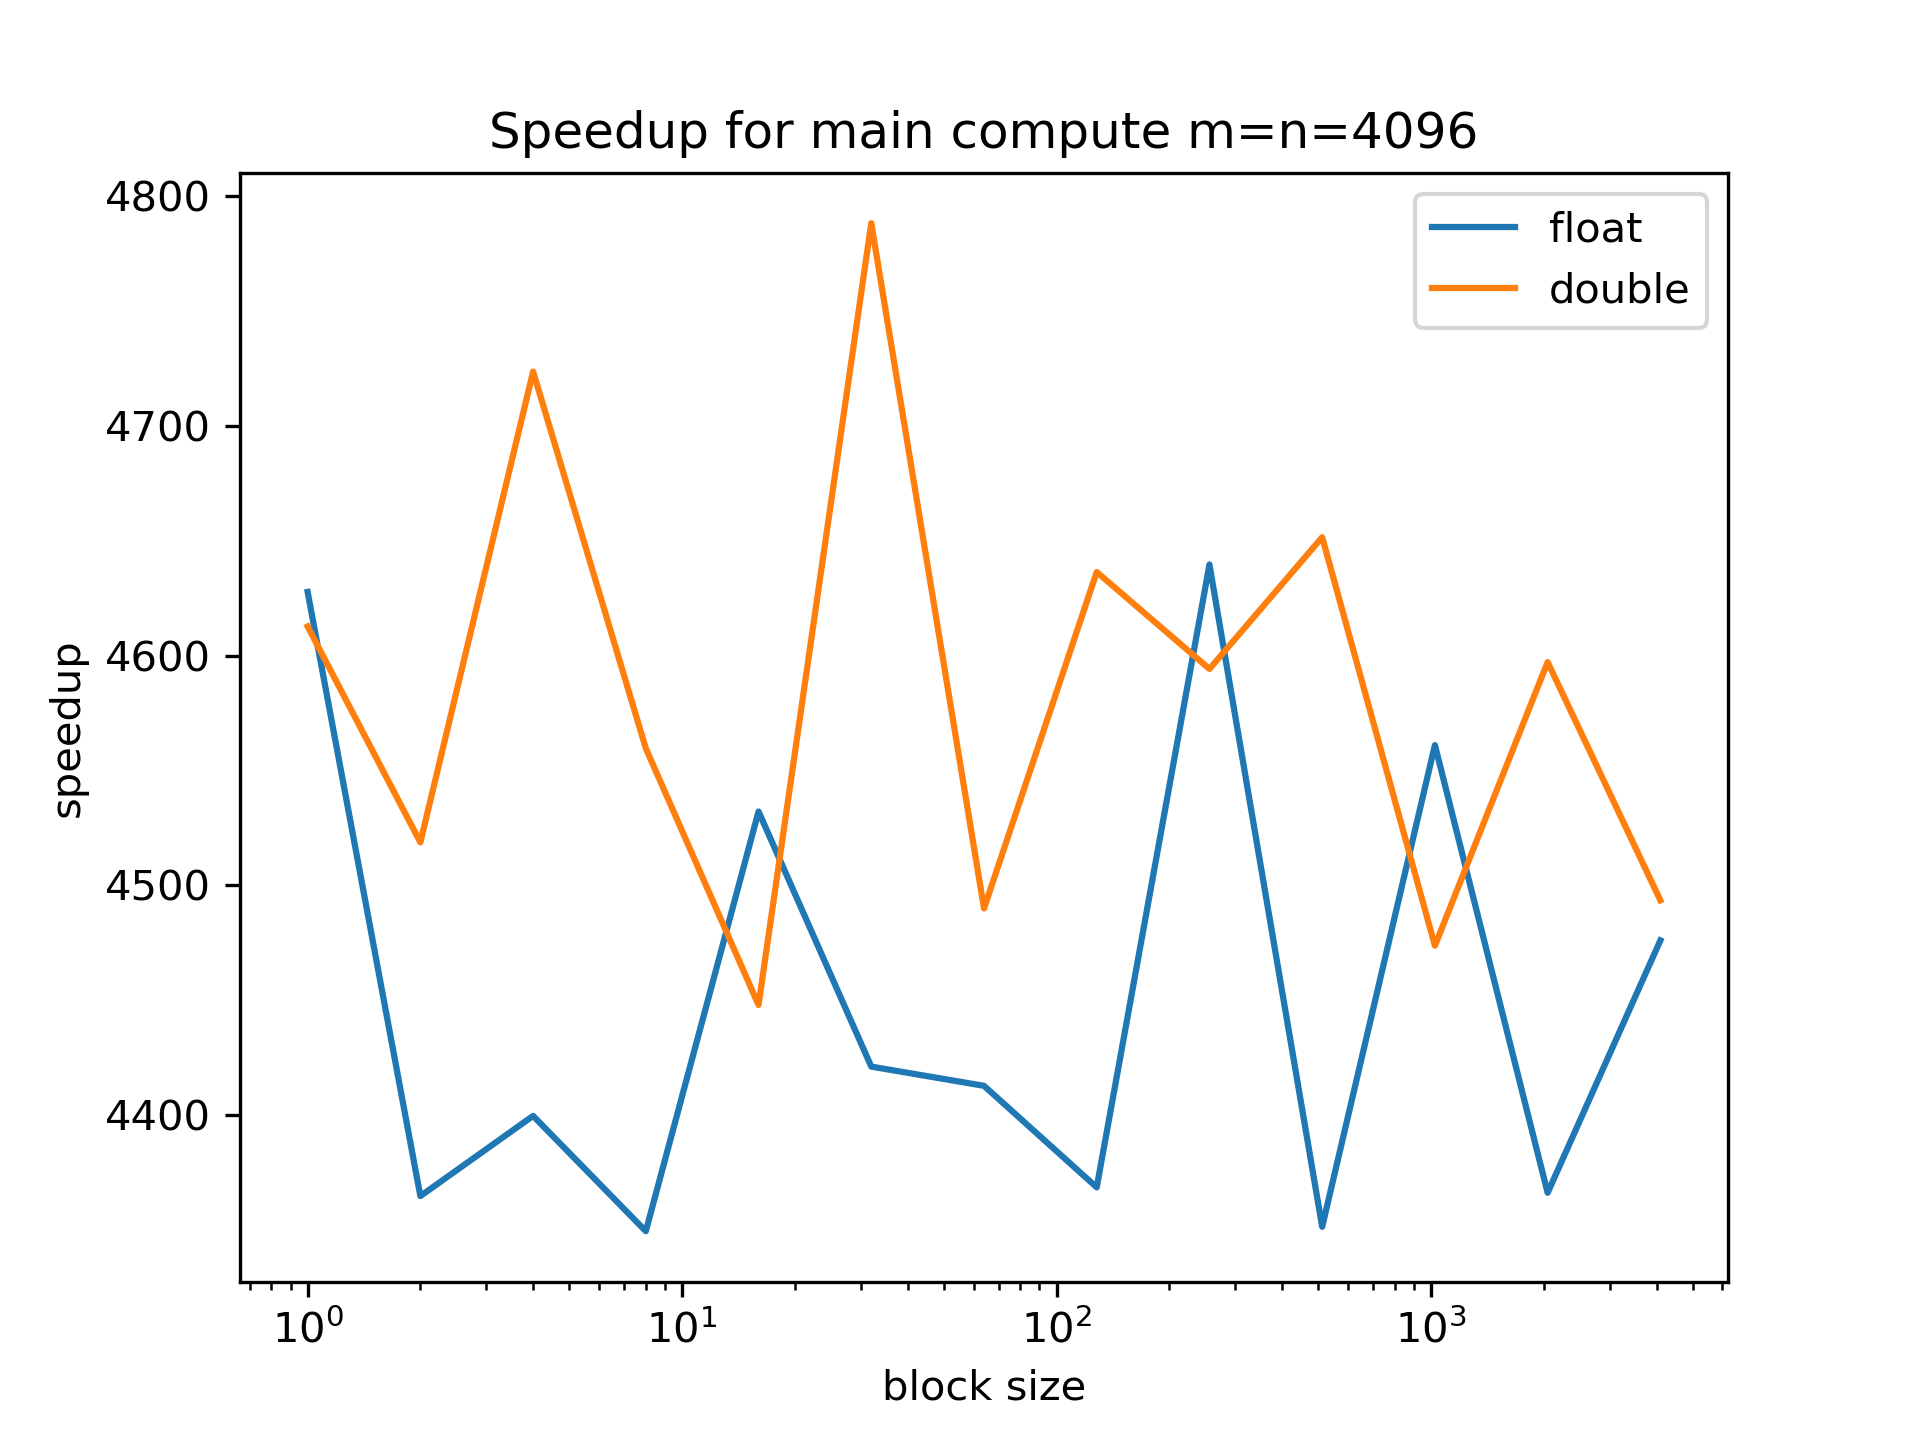
\includegraphics[width=\linewidth]{../comparison_plots/compute_plot_m4096.png}
		\end{minipage}%
		\begin{minipage}{0.45\linewidth}
			\centering
			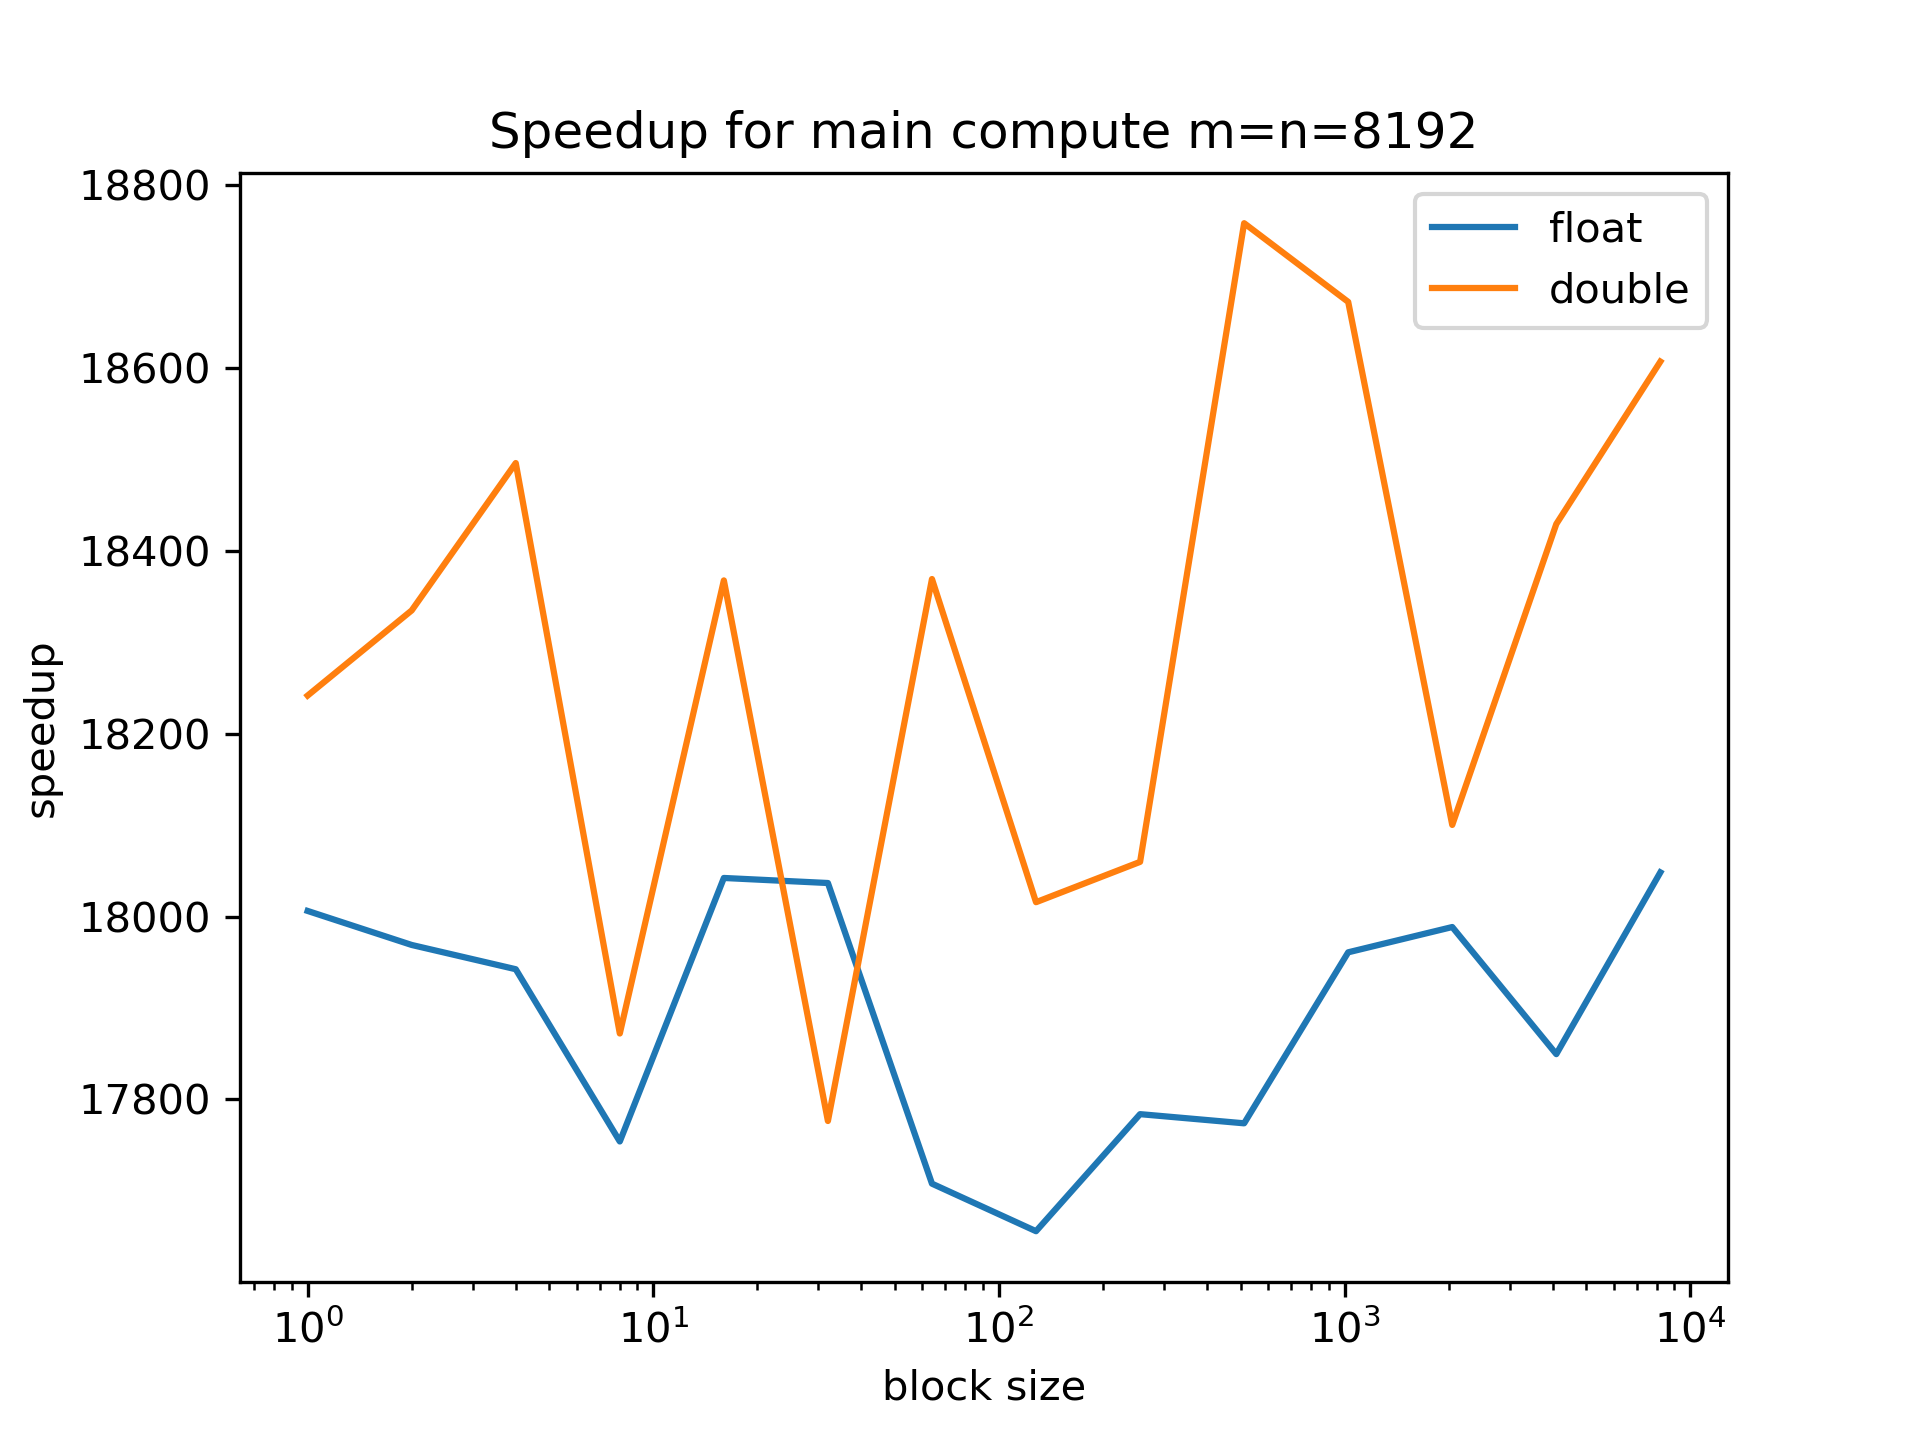
\includegraphics[width=\linewidth]{../comparison_plots/compute_plot_m8192.png}
		\end{minipage}
	\end{figure}


	\begin{figure}[h!]
		\centering
		\begin{minipage}{0.45\linewidth}
			\centering
			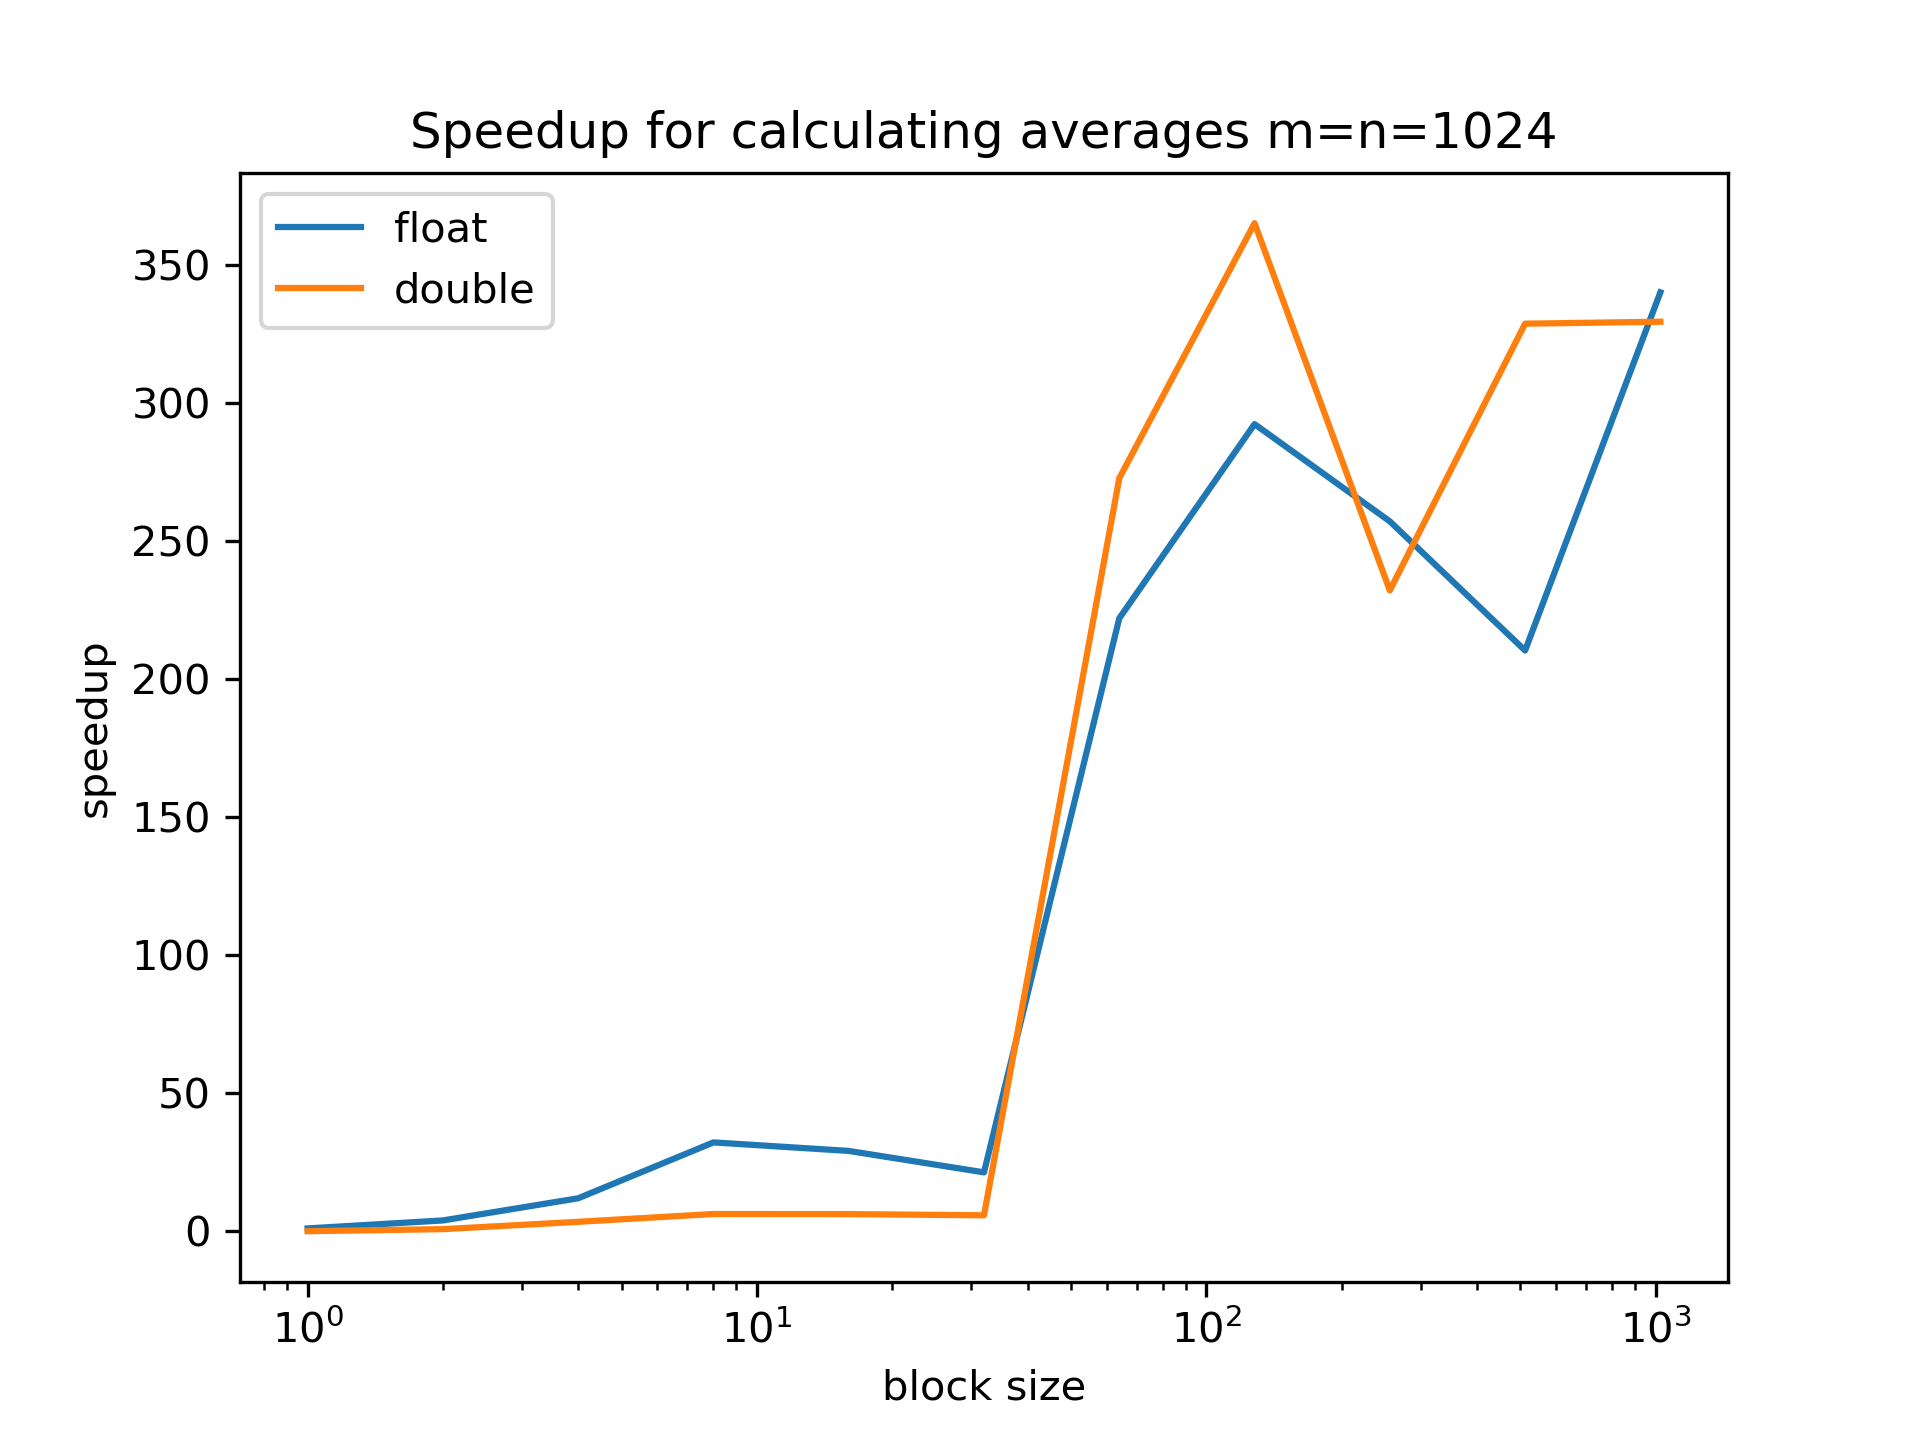
\includegraphics[width=\linewidth]{../comparison_plots/reduce_plot_m1024.png}
		\end{minipage}%
		\begin{minipage}{0.45\linewidth}
			\centering
			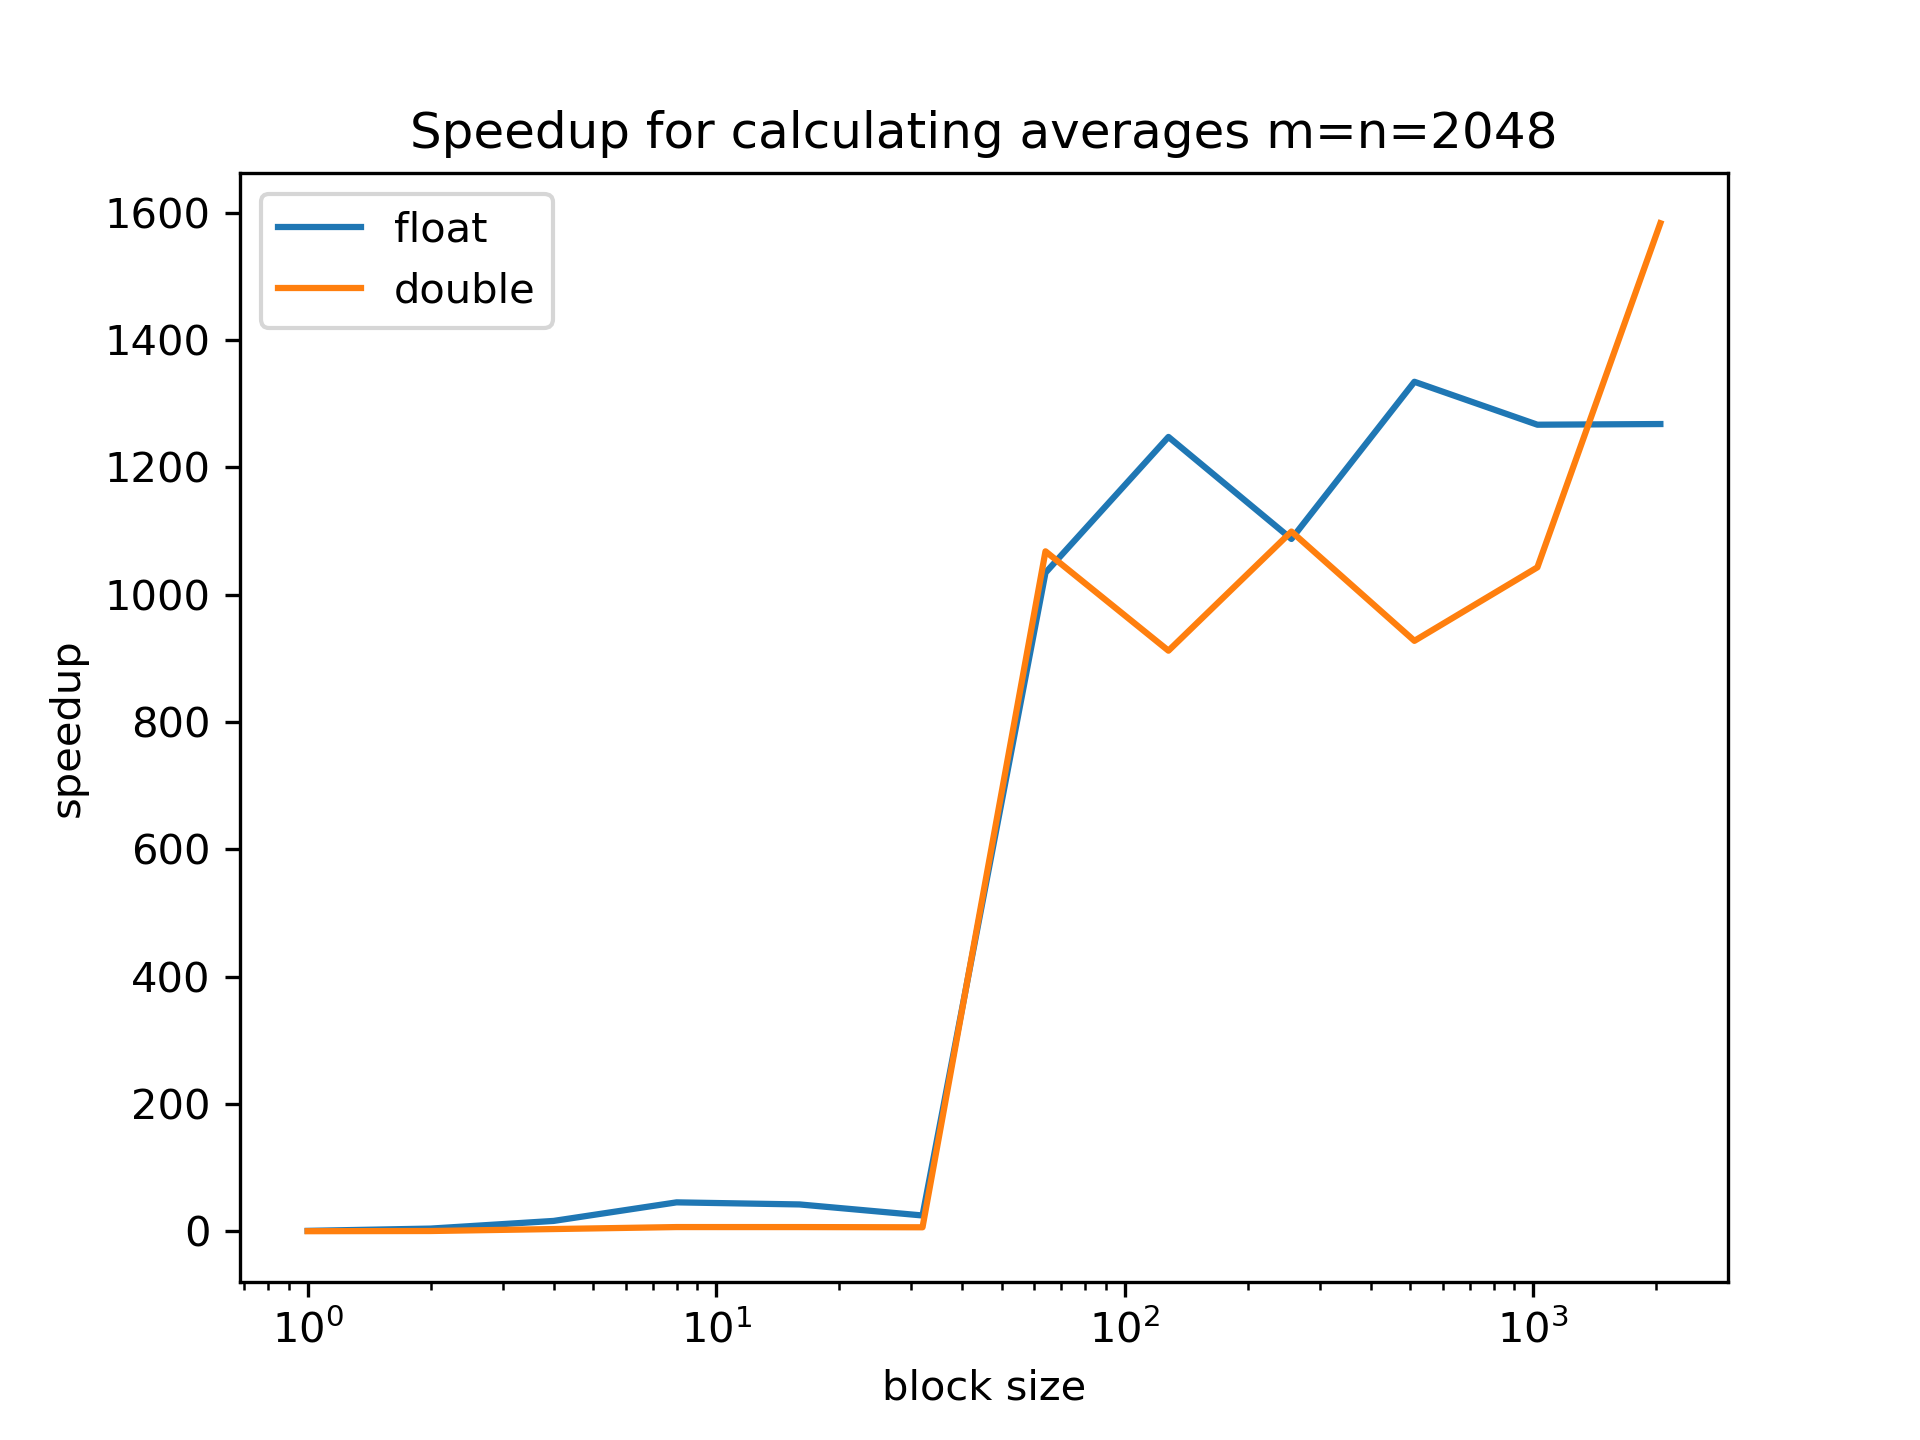
\includegraphics[width=\linewidth]{../comparison_plots/reduce_plot_m2048.png}
		\end{minipage}
		\vspace{0.5cm} % Adjust the vertical space between rows
		\begin{minipage}{0.45\linewidth}
			\centering
			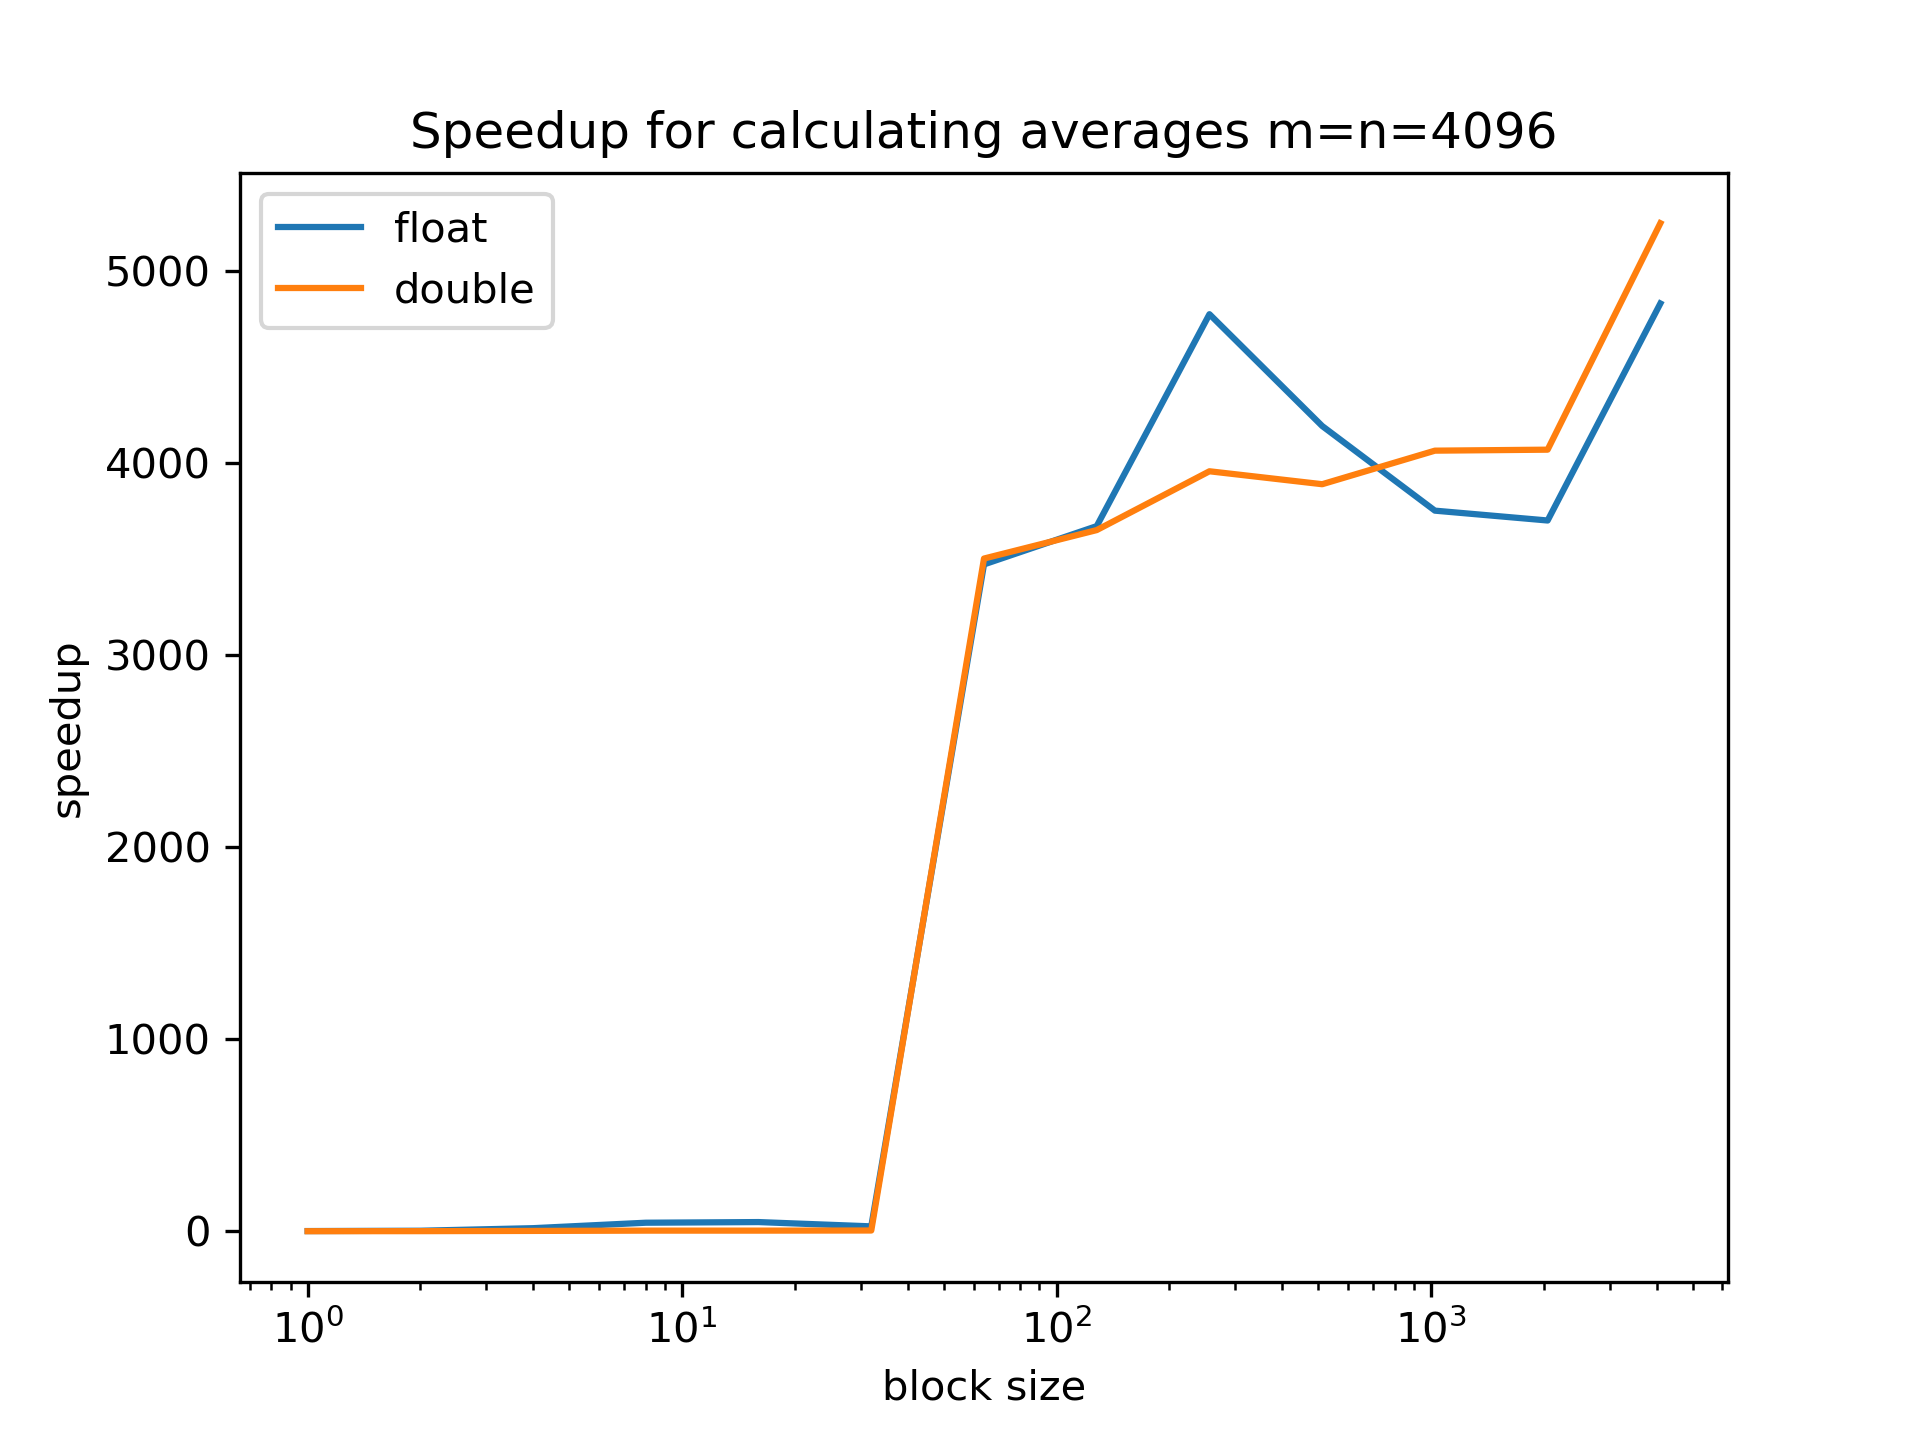
\includegraphics[width=\linewidth]{../comparison_plots/reduce_plot_m4096.png}
		\end{minipage}%
		\begin{minipage}{0.45\linewidth}
			\centering
			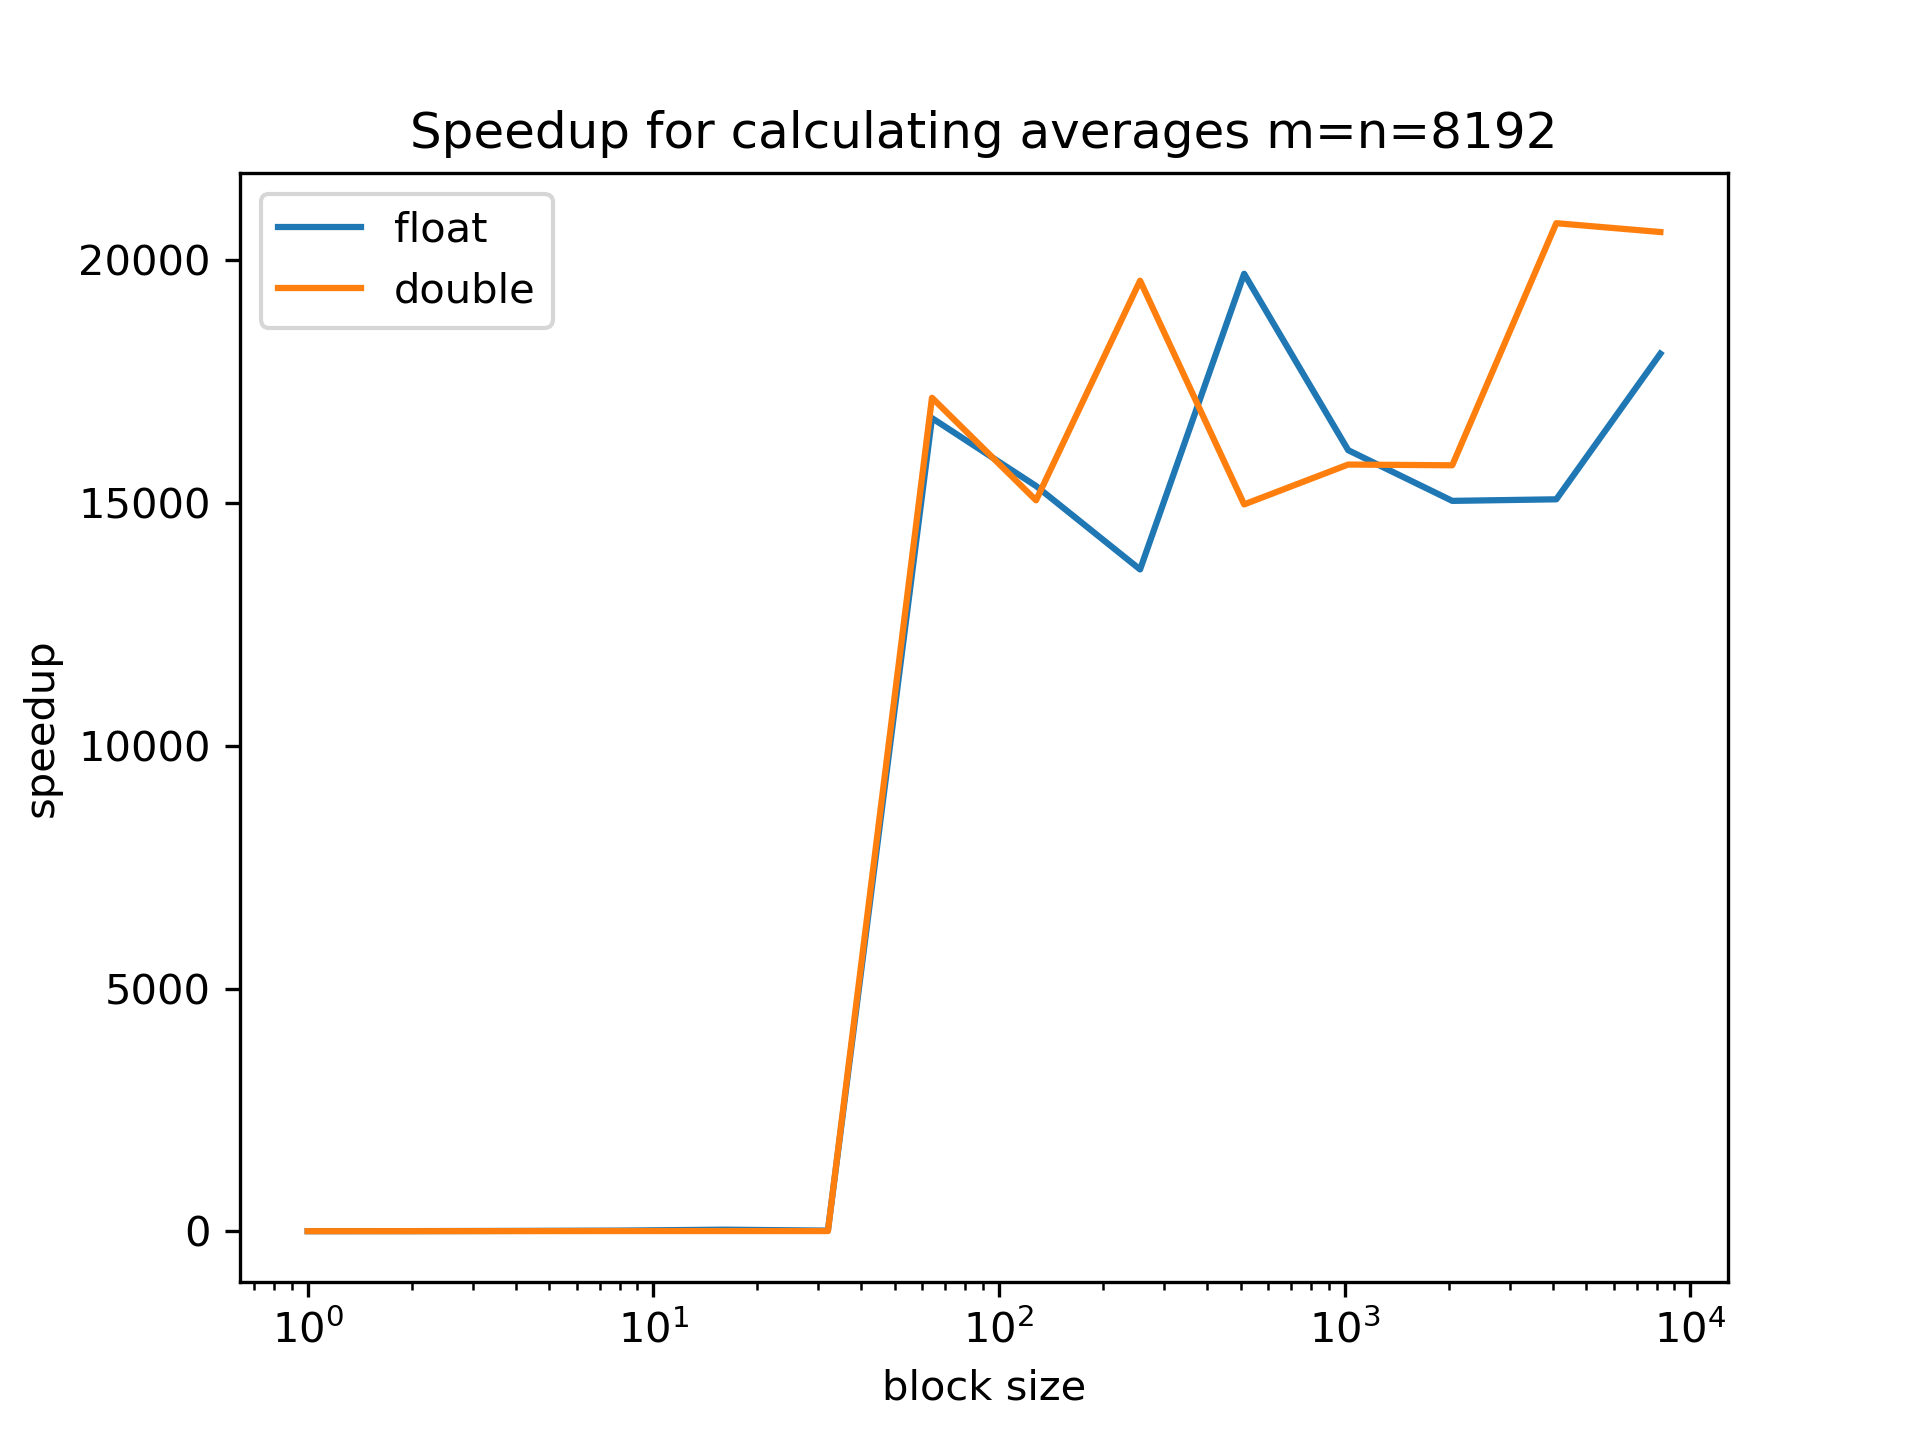
\includegraphics[width=\linewidth]{../comparison_plots/reduce_plot_m8192.png}
		\end{minipage}
	\end{figure}

\bibliographystyle{plain}
\bibliography{refs}

\end{document}

